
% Default to the notebook output style

    


% Inherit from the specified cell style.




    
\documentclass[11pt]{article}

    
    
    \usepackage[T1]{fontenc}
    % Nicer default font (+ math font) than Computer Modern for most use cases
    \usepackage{mathpazo}

    % Basic figure setup, for now with no caption control since it's done
    % automatically by Pandoc (which extracts ![](path) syntax from Markdown).
    \usepackage{graphicx}
    % We will generate all images so they have a width \maxwidth. This means
    % that they will get their normal width if they fit onto the page, but
    % are scaled down if they would overflow the margins.
    \makeatletter
    \def\maxwidth{\ifdim\Gin@nat@width>\linewidth\linewidth
    \else\Gin@nat@width\fi}
    \makeatother
    \let\Oldincludegraphics\includegraphics
    % Set max figure width to be 80% of text width, for now hardcoded.
    \renewcommand{\includegraphics}[1]{\Oldincludegraphics[width=.8\maxwidth]{#1}}
    % Ensure that by default, figures have no caption (until we provide a
    % proper Figure object with a Caption API and a way to capture that
    % in the conversion process - todo).
    \usepackage{caption}
    \DeclareCaptionLabelFormat{nolabel}{}
    \captionsetup{labelformat=nolabel}

    \usepackage{adjustbox} % Used to constrain images to a maximum size 
    \usepackage{xcolor} % Allow colors to be defined
    \usepackage{enumerate} % Needed for markdown enumerations to work
    \usepackage{geometry} % Used to adjust the document margins
    \usepackage{amsmath} % Equations
    \usepackage{amssymb} % Equations
    \usepackage{textcomp} % defines textquotesingle
    % Hack from http://tex.stackexchange.com/a/47451/13684:
    \AtBeginDocument{%
        \def\PYZsq{\textquotesingle}% Upright quotes in Pygmentized code
    }
    \usepackage{upquote} % Upright quotes for verbatim code
    \usepackage{eurosym} % defines \euro
    \usepackage[mathletters]{ucs} % Extended unicode (utf-8) support
    \usepackage[utf8x]{inputenc} % Allow utf-8 characters in the tex document
    \usepackage{fancyvrb} % verbatim replacement that allows latex
    \usepackage{grffile} % extends the file name processing of package graphics 
                         % to support a larger range 
    % The hyperref package gives us a pdf with properly built
    % internal navigation ('pdf bookmarks' for the table of contents,
    % internal cross-reference links, web links for URLs, etc.)
    \usepackage{hyperref}
    \usepackage{longtable} % longtable support required by pandoc >1.10
    \usepackage{booktabs}  % table support for pandoc > 1.12.2
    \usepackage[inline]{enumitem} % IRkernel/repr support (it uses the enumerate* environment)
    \usepackage[normalem]{ulem} % ulem is needed to support strikethroughs (\sout)
                                % normalem makes italics be italics, not underlines
    

    
    
    % Colors for the hyperref package
    \definecolor{urlcolor}{rgb}{0,.145,.698}
    \definecolor{linkcolor}{rgb}{.71,0.21,0.01}
    \definecolor{citecolor}{rgb}{.12,.54,.11}

    % ANSI colors
    \definecolor{ansi-black}{HTML}{3E424D}
    \definecolor{ansi-black-intense}{HTML}{282C36}
    \definecolor{ansi-red}{HTML}{E75C58}
    \definecolor{ansi-red-intense}{HTML}{B22B31}
    \definecolor{ansi-green}{HTML}{00A250}
    \definecolor{ansi-green-intense}{HTML}{007427}
    \definecolor{ansi-yellow}{HTML}{DDB62B}
    \definecolor{ansi-yellow-intense}{HTML}{B27D12}
    \definecolor{ansi-blue}{HTML}{208FFB}
    \definecolor{ansi-blue-intense}{HTML}{0065CA}
    \definecolor{ansi-magenta}{HTML}{D160C4}
    \definecolor{ansi-magenta-intense}{HTML}{A03196}
    \definecolor{ansi-cyan}{HTML}{60C6C8}
    \definecolor{ansi-cyan-intense}{HTML}{258F8F}
    \definecolor{ansi-white}{HTML}{C5C1B4}
    \definecolor{ansi-white-intense}{HTML}{A1A6B2}

    % commands and environments needed by pandoc snippets
    % extracted from the output of `pandoc -s`
    \providecommand{\tightlist}{%
      \setlength{\itemsep}{0pt}\setlength{\parskip}{0pt}}
    \DefineVerbatimEnvironment{Highlighting}{Verbatim}{commandchars=\\\{\}}
    % Add ',fontsize=\small' for more characters per line
    \newenvironment{Shaded}{}{}
    \newcommand{\KeywordTok}[1]{\textcolor[rgb]{0.00,0.44,0.13}{\textbf{{#1}}}}
    \newcommand{\DataTypeTok}[1]{\textcolor[rgb]{0.56,0.13,0.00}{{#1}}}
    \newcommand{\DecValTok}[1]{\textcolor[rgb]{0.25,0.63,0.44}{{#1}}}
    \newcommand{\BaseNTok}[1]{\textcolor[rgb]{0.25,0.63,0.44}{{#1}}}
    \newcommand{\FloatTok}[1]{\textcolor[rgb]{0.25,0.63,0.44}{{#1}}}
    \newcommand{\CharTok}[1]{\textcolor[rgb]{0.25,0.44,0.63}{{#1}}}
    \newcommand{\StringTok}[1]{\textcolor[rgb]{0.25,0.44,0.63}{{#1}}}
    \newcommand{\CommentTok}[1]{\textcolor[rgb]{0.38,0.63,0.69}{\textit{{#1}}}}
    \newcommand{\OtherTok}[1]{\textcolor[rgb]{0.00,0.44,0.13}{{#1}}}
    \newcommand{\AlertTok}[1]{\textcolor[rgb]{1.00,0.00,0.00}{\textbf{{#1}}}}
    \newcommand{\FunctionTok}[1]{\textcolor[rgb]{0.02,0.16,0.49}{{#1}}}
    \newcommand{\RegionMarkerTok}[1]{{#1}}
    \newcommand{\ErrorTok}[1]{\textcolor[rgb]{1.00,0.00,0.00}{\textbf{{#1}}}}
    \newcommand{\NormalTok}[1]{{#1}}
    
    % Additional commands for more recent versions of Pandoc
    \newcommand{\ConstantTok}[1]{\textcolor[rgb]{0.53,0.00,0.00}{{#1}}}
    \newcommand{\SpecialCharTok}[1]{\textcolor[rgb]{0.25,0.44,0.63}{{#1}}}
    \newcommand{\VerbatimStringTok}[1]{\textcolor[rgb]{0.25,0.44,0.63}{{#1}}}
    \newcommand{\SpecialStringTok}[1]{\textcolor[rgb]{0.73,0.40,0.53}{{#1}}}
    \newcommand{\ImportTok}[1]{{#1}}
    \newcommand{\DocumentationTok}[1]{\textcolor[rgb]{0.73,0.13,0.13}{\textit{{#1}}}}
    \newcommand{\AnnotationTok}[1]{\textcolor[rgb]{0.38,0.63,0.69}{\textbf{\textit{{#1}}}}}
    \newcommand{\CommentVarTok}[1]{\textcolor[rgb]{0.38,0.63,0.69}{\textbf{\textit{{#1}}}}}
    \newcommand{\VariableTok}[1]{\textcolor[rgb]{0.10,0.09,0.49}{{#1}}}
    \newcommand{\ControlFlowTok}[1]{\textcolor[rgb]{0.00,0.44,0.13}{\textbf{{#1}}}}
    \newcommand{\OperatorTok}[1]{\textcolor[rgb]{0.40,0.40,0.40}{{#1}}}
    \newcommand{\BuiltInTok}[1]{{#1}}
    \newcommand{\ExtensionTok}[1]{{#1}}
    \newcommand{\PreprocessorTok}[1]{\textcolor[rgb]{0.74,0.48,0.00}{{#1}}}
    \newcommand{\AttributeTok}[1]{\textcolor[rgb]{0.49,0.56,0.16}{{#1}}}
    \newcommand{\InformationTok}[1]{\textcolor[rgb]{0.38,0.63,0.69}{\textbf{\textit{{#1}}}}}
    \newcommand{\WarningTok}[1]{\textcolor[rgb]{0.38,0.63,0.69}{\textbf{\textit{{#1}}}}}
    
    
    % Define a nice break command that doesn't care if a line doesn't already
    % exist.
    \def\br{\hspace*{\fill} \\* }
    % Math Jax compatability definitions
    \def\gt{>}
    \def\lt{<}
    % Document parameters
    \title{Assignment 4}
    
    
    

    % Pygments definitions
    
\makeatletter
\def\PY@reset{\let\PY@it=\relax \let\PY@bf=\relax%
    \let\PY@ul=\relax \let\PY@tc=\relax%
    \let\PY@bc=\relax \let\PY@ff=\relax}
\def\PY@tok#1{\csname PY@tok@#1\endcsname}
\def\PY@toks#1+{\ifx\relax#1\empty\else%
    \PY@tok{#1}\expandafter\PY@toks\fi}
\def\PY@do#1{\PY@bc{\PY@tc{\PY@ul{%
    \PY@it{\PY@bf{\PY@ff{#1}}}}}}}
\def\PY#1#2{\PY@reset\PY@toks#1+\relax+\PY@do{#2}}

\expandafter\def\csname PY@tok@w\endcsname{\def\PY@tc##1{\textcolor[rgb]{0.73,0.73,0.73}{##1}}}
\expandafter\def\csname PY@tok@c\endcsname{\let\PY@it=\textit\def\PY@tc##1{\textcolor[rgb]{0.25,0.50,0.50}{##1}}}
\expandafter\def\csname PY@tok@cp\endcsname{\def\PY@tc##1{\textcolor[rgb]{0.74,0.48,0.00}{##1}}}
\expandafter\def\csname PY@tok@k\endcsname{\let\PY@bf=\textbf\def\PY@tc##1{\textcolor[rgb]{0.00,0.50,0.00}{##1}}}
\expandafter\def\csname PY@tok@kp\endcsname{\def\PY@tc##1{\textcolor[rgb]{0.00,0.50,0.00}{##1}}}
\expandafter\def\csname PY@tok@kt\endcsname{\def\PY@tc##1{\textcolor[rgb]{0.69,0.00,0.25}{##1}}}
\expandafter\def\csname PY@tok@o\endcsname{\def\PY@tc##1{\textcolor[rgb]{0.40,0.40,0.40}{##1}}}
\expandafter\def\csname PY@tok@ow\endcsname{\let\PY@bf=\textbf\def\PY@tc##1{\textcolor[rgb]{0.67,0.13,1.00}{##1}}}
\expandafter\def\csname PY@tok@nb\endcsname{\def\PY@tc##1{\textcolor[rgb]{0.00,0.50,0.00}{##1}}}
\expandafter\def\csname PY@tok@nf\endcsname{\def\PY@tc##1{\textcolor[rgb]{0.00,0.00,1.00}{##1}}}
\expandafter\def\csname PY@tok@nc\endcsname{\let\PY@bf=\textbf\def\PY@tc##1{\textcolor[rgb]{0.00,0.00,1.00}{##1}}}
\expandafter\def\csname PY@tok@nn\endcsname{\let\PY@bf=\textbf\def\PY@tc##1{\textcolor[rgb]{0.00,0.00,1.00}{##1}}}
\expandafter\def\csname PY@tok@ne\endcsname{\let\PY@bf=\textbf\def\PY@tc##1{\textcolor[rgb]{0.82,0.25,0.23}{##1}}}
\expandafter\def\csname PY@tok@nv\endcsname{\def\PY@tc##1{\textcolor[rgb]{0.10,0.09,0.49}{##1}}}
\expandafter\def\csname PY@tok@no\endcsname{\def\PY@tc##1{\textcolor[rgb]{0.53,0.00,0.00}{##1}}}
\expandafter\def\csname PY@tok@nl\endcsname{\def\PY@tc##1{\textcolor[rgb]{0.63,0.63,0.00}{##1}}}
\expandafter\def\csname PY@tok@ni\endcsname{\let\PY@bf=\textbf\def\PY@tc##1{\textcolor[rgb]{0.60,0.60,0.60}{##1}}}
\expandafter\def\csname PY@tok@na\endcsname{\def\PY@tc##1{\textcolor[rgb]{0.49,0.56,0.16}{##1}}}
\expandafter\def\csname PY@tok@nt\endcsname{\let\PY@bf=\textbf\def\PY@tc##1{\textcolor[rgb]{0.00,0.50,0.00}{##1}}}
\expandafter\def\csname PY@tok@nd\endcsname{\def\PY@tc##1{\textcolor[rgb]{0.67,0.13,1.00}{##1}}}
\expandafter\def\csname PY@tok@s\endcsname{\def\PY@tc##1{\textcolor[rgb]{0.73,0.13,0.13}{##1}}}
\expandafter\def\csname PY@tok@sd\endcsname{\let\PY@it=\textit\def\PY@tc##1{\textcolor[rgb]{0.73,0.13,0.13}{##1}}}
\expandafter\def\csname PY@tok@si\endcsname{\let\PY@bf=\textbf\def\PY@tc##1{\textcolor[rgb]{0.73,0.40,0.53}{##1}}}
\expandafter\def\csname PY@tok@se\endcsname{\let\PY@bf=\textbf\def\PY@tc##1{\textcolor[rgb]{0.73,0.40,0.13}{##1}}}
\expandafter\def\csname PY@tok@sr\endcsname{\def\PY@tc##1{\textcolor[rgb]{0.73,0.40,0.53}{##1}}}
\expandafter\def\csname PY@tok@ss\endcsname{\def\PY@tc##1{\textcolor[rgb]{0.10,0.09,0.49}{##1}}}
\expandafter\def\csname PY@tok@sx\endcsname{\def\PY@tc##1{\textcolor[rgb]{0.00,0.50,0.00}{##1}}}
\expandafter\def\csname PY@tok@m\endcsname{\def\PY@tc##1{\textcolor[rgb]{0.40,0.40,0.40}{##1}}}
\expandafter\def\csname PY@tok@gh\endcsname{\let\PY@bf=\textbf\def\PY@tc##1{\textcolor[rgb]{0.00,0.00,0.50}{##1}}}
\expandafter\def\csname PY@tok@gu\endcsname{\let\PY@bf=\textbf\def\PY@tc##1{\textcolor[rgb]{0.50,0.00,0.50}{##1}}}
\expandafter\def\csname PY@tok@gd\endcsname{\def\PY@tc##1{\textcolor[rgb]{0.63,0.00,0.00}{##1}}}
\expandafter\def\csname PY@tok@gi\endcsname{\def\PY@tc##1{\textcolor[rgb]{0.00,0.63,0.00}{##1}}}
\expandafter\def\csname PY@tok@gr\endcsname{\def\PY@tc##1{\textcolor[rgb]{1.00,0.00,0.00}{##1}}}
\expandafter\def\csname PY@tok@ge\endcsname{\let\PY@it=\textit}
\expandafter\def\csname PY@tok@gs\endcsname{\let\PY@bf=\textbf}
\expandafter\def\csname PY@tok@gp\endcsname{\let\PY@bf=\textbf\def\PY@tc##1{\textcolor[rgb]{0.00,0.00,0.50}{##1}}}
\expandafter\def\csname PY@tok@go\endcsname{\def\PY@tc##1{\textcolor[rgb]{0.53,0.53,0.53}{##1}}}
\expandafter\def\csname PY@tok@gt\endcsname{\def\PY@tc##1{\textcolor[rgb]{0.00,0.27,0.87}{##1}}}
\expandafter\def\csname PY@tok@err\endcsname{\def\PY@bc##1{\setlength{\fboxsep}{0pt}\fcolorbox[rgb]{1.00,0.00,0.00}{1,1,1}{\strut ##1}}}
\expandafter\def\csname PY@tok@kc\endcsname{\let\PY@bf=\textbf\def\PY@tc##1{\textcolor[rgb]{0.00,0.50,0.00}{##1}}}
\expandafter\def\csname PY@tok@kd\endcsname{\let\PY@bf=\textbf\def\PY@tc##1{\textcolor[rgb]{0.00,0.50,0.00}{##1}}}
\expandafter\def\csname PY@tok@kn\endcsname{\let\PY@bf=\textbf\def\PY@tc##1{\textcolor[rgb]{0.00,0.50,0.00}{##1}}}
\expandafter\def\csname PY@tok@kr\endcsname{\let\PY@bf=\textbf\def\PY@tc##1{\textcolor[rgb]{0.00,0.50,0.00}{##1}}}
\expandafter\def\csname PY@tok@bp\endcsname{\def\PY@tc##1{\textcolor[rgb]{0.00,0.50,0.00}{##1}}}
\expandafter\def\csname PY@tok@fm\endcsname{\def\PY@tc##1{\textcolor[rgb]{0.00,0.00,1.00}{##1}}}
\expandafter\def\csname PY@tok@vc\endcsname{\def\PY@tc##1{\textcolor[rgb]{0.10,0.09,0.49}{##1}}}
\expandafter\def\csname PY@tok@vg\endcsname{\def\PY@tc##1{\textcolor[rgb]{0.10,0.09,0.49}{##1}}}
\expandafter\def\csname PY@tok@vi\endcsname{\def\PY@tc##1{\textcolor[rgb]{0.10,0.09,0.49}{##1}}}
\expandafter\def\csname PY@tok@vm\endcsname{\def\PY@tc##1{\textcolor[rgb]{0.10,0.09,0.49}{##1}}}
\expandafter\def\csname PY@tok@sa\endcsname{\def\PY@tc##1{\textcolor[rgb]{0.73,0.13,0.13}{##1}}}
\expandafter\def\csname PY@tok@sb\endcsname{\def\PY@tc##1{\textcolor[rgb]{0.73,0.13,0.13}{##1}}}
\expandafter\def\csname PY@tok@sc\endcsname{\def\PY@tc##1{\textcolor[rgb]{0.73,0.13,0.13}{##1}}}
\expandafter\def\csname PY@tok@dl\endcsname{\def\PY@tc##1{\textcolor[rgb]{0.73,0.13,0.13}{##1}}}
\expandafter\def\csname PY@tok@s2\endcsname{\def\PY@tc##1{\textcolor[rgb]{0.73,0.13,0.13}{##1}}}
\expandafter\def\csname PY@tok@sh\endcsname{\def\PY@tc##1{\textcolor[rgb]{0.73,0.13,0.13}{##1}}}
\expandafter\def\csname PY@tok@s1\endcsname{\def\PY@tc##1{\textcolor[rgb]{0.73,0.13,0.13}{##1}}}
\expandafter\def\csname PY@tok@mb\endcsname{\def\PY@tc##1{\textcolor[rgb]{0.40,0.40,0.40}{##1}}}
\expandafter\def\csname PY@tok@mf\endcsname{\def\PY@tc##1{\textcolor[rgb]{0.40,0.40,0.40}{##1}}}
\expandafter\def\csname PY@tok@mh\endcsname{\def\PY@tc##1{\textcolor[rgb]{0.40,0.40,0.40}{##1}}}
\expandafter\def\csname PY@tok@mi\endcsname{\def\PY@tc##1{\textcolor[rgb]{0.40,0.40,0.40}{##1}}}
\expandafter\def\csname PY@tok@il\endcsname{\def\PY@tc##1{\textcolor[rgb]{0.40,0.40,0.40}{##1}}}
\expandafter\def\csname PY@tok@mo\endcsname{\def\PY@tc##1{\textcolor[rgb]{0.40,0.40,0.40}{##1}}}
\expandafter\def\csname PY@tok@ch\endcsname{\let\PY@it=\textit\def\PY@tc##1{\textcolor[rgb]{0.25,0.50,0.50}{##1}}}
\expandafter\def\csname PY@tok@cm\endcsname{\let\PY@it=\textit\def\PY@tc##1{\textcolor[rgb]{0.25,0.50,0.50}{##1}}}
\expandafter\def\csname PY@tok@cpf\endcsname{\let\PY@it=\textit\def\PY@tc##1{\textcolor[rgb]{0.25,0.50,0.50}{##1}}}
\expandafter\def\csname PY@tok@c1\endcsname{\let\PY@it=\textit\def\PY@tc##1{\textcolor[rgb]{0.25,0.50,0.50}{##1}}}
\expandafter\def\csname PY@tok@cs\endcsname{\let\PY@it=\textit\def\PY@tc##1{\textcolor[rgb]{0.25,0.50,0.50}{##1}}}

\def\PYZbs{\char`\\}
\def\PYZus{\char`\_}
\def\PYZob{\char`\{}
\def\PYZcb{\char`\}}
\def\PYZca{\char`\^}
\def\PYZam{\char`\&}
\def\PYZlt{\char`\<}
\def\PYZgt{\char`\>}
\def\PYZsh{\char`\#}
\def\PYZpc{\char`\%}
\def\PYZdl{\char`\$}
\def\PYZhy{\char`\-}
\def\PYZsq{\char`\'}
\def\PYZdq{\char`\"}
\def\PYZti{\char`\~}
% for compatibility with earlier versions
\def\PYZat{@}
\def\PYZlb{[}
\def\PYZrb{]}
\makeatother


    % Exact colors from NB
    \definecolor{incolor}{rgb}{0.0, 0.0, 0.5}
    \definecolor{outcolor}{rgb}{0.545, 0.0, 0.0}



    
    % Prevent overflowing lines due to hard-to-break entities
    \sloppy 
    % Setup hyperref package
    \hypersetup{
      breaklinks=true,  % so long urls are correctly broken across lines
      colorlinks=true,
      urlcolor=urlcolor,
      linkcolor=linkcolor,
      citecolor=citecolor,
      }
    % Slightly bigger margins than the latex defaults
    
    \geometry{verbose,tmargin=1in,bmargin=1in,lmargin=1in,rmargin=1in}
    
    

    \begin{document}
    
    
    \maketitle
    
    

    
    \hypertarget{phys-581-winter-2019}{%
\section{Phys 581 Winter 2019}\label{phys-581-winter-2019}}

\hypertarget{assignment-4-neural-networks}{%
\section{Assignment \#4: Neural
Networks}\label{assignment-4-neural-networks}}

\hypertarget{alexander-hickey-10169582}{%
\subsection{Alexander Hickey,
10169582}\label{alexander-hickey-10169582}}

    Note that this notebook makes use of the Keras deep learning library for
python, which is compatible only with Python 2.7-3.6.

    \begin{Verbatim}[commandchars=\\\{\}]
{\color{incolor}In [{\color{incolor}1}]:} \PY{c+c1}{\PYZsh{}Must be running Python 3.6 or lower!}
        \PY{k+kn}{import} \PY{n+nn}{sys}
        \PY{n}{sys}\PY{o}{.}\PY{n}{version}
\end{Verbatim}


\begin{Verbatim}[commandchars=\\\{\}]
{\color{outcolor}Out[{\color{outcolor}1}]:} '3.6.8 |Anaconda, Inc.| (default, Feb 21 2019, 18:30:04) [MSC v.1916 64 bit (AMD64)]'
\end{Verbatim}
            
    \begin{Verbatim}[commandchars=\\\{\}]
{\color{incolor}In [{\color{incolor}2}]:} \PY{c+c1}{\PYZsh{}Import useful libraries}
        \PY{k+kn}{import} \PY{n+nn}{numpy} \PY{k}{as} \PY{n+nn}{np}
        \PY{k+kn}{import} \PY{n+nn}{matplotlib}\PY{n+nn}{.}\PY{n+nn}{pyplot} \PY{k}{as} \PY{n+nn}{plt}
        \PY{k+kn}{from} \PY{n+nn}{mpl\PYZus{}toolkits}\PY{n+nn}{.}\PY{n+nn}{mplot3d} \PY{k}{import} \PY{n}{Axes3D}
        \PY{k+kn}{import} \PY{n+nn}{scipy}\PY{n+nn}{.}\PY{n+nn}{integrate}
        \PY{k+kn}{from} \PY{n+nn}{keras}\PY{n+nn}{.}\PY{n+nn}{models} \PY{k}{import} \PY{n}{Model}\PY{p}{,} \PY{n}{Sequential}
        \PY{k+kn}{from} \PY{n+nn}{keras}\PY{n+nn}{.}\PY{n+nn}{layers} \PY{k}{import} \PY{n}{Input}\PY{p}{,} \PY{n}{Dense}
        \PY{k+kn}{from} \PY{n+nn}{keras}\PY{n+nn}{.}\PY{n+nn}{backend} \PY{k}{import} \PY{n}{clear\PYZus{}session}
        \PY{o}{\PYZpc{}}\PY{k}{matplotlib} inline
\end{Verbatim}


    \begin{Verbatim}[commandchars=\\\{\}]
Using TensorFlow backend.

    \end{Verbatim}

    \hypertarget{introduction}{%
\subsubsection{Introduction}\label{introduction}}

    Inspired by biological neural networks, a method of machine learning
known as deep learning has revolutionized the way that scientists model
complex systems. In general, a neural network is a collection of
connected nodes (or \emph{neurons}) that can transmit data through their
connections (or \emph{edges}). Typically, the neurons are oraganized
into layers, each of which can perform different kings of
transformations on their inputs. Additionally, each of the edges are
assigned a weight that increases or decreases the strength of a signal
at an edge, and these weights are adjusted in the learning process using
a set of training data. The term \emph{deep} neural network refers to a
neural network with more than one hidden layer (see Figure below).

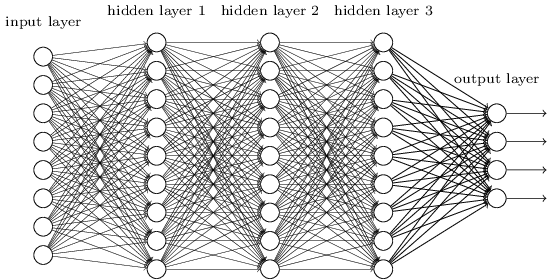
\includegraphics{tikz41.png} (Image source:
http://neuralnetworksanddeeplearning.com/chap6.html)

Recently, there has been great interest in the use of machine learning
to predict solutions of physical problems, such as the solutions of a
non-linear system of differential equations. In this notebook, we will
explore the implementation of machine learning to predict the time
evolution of the Lorenz system, which is notable for producing chaotic
solutions under certain parameter ranges. The Lorenz equations are:

\begin{align*}
\frac{dx}{dt} &= \sigma(y-x) \\
\frac{dy}{dt} &= x(\rho-z)-y \\
\frac{dz}{dt} &= xy-\beta z
\end{align*}

For the choice of parameters \((\sigma,\beta,\rho) = (10,8/3,58)\), it
is known that the solution is a ``butterfly'' like strange attractor
that exhibits deterministic chaos. The goal of this work will be to
construct and train a neural network that takes a solution set of the
Lorenz equations over some time interval \([0,t]\), and predicts the
solution set over some shifted time interval \([\Delta t,t+ \Delta t]\).
This will be done through the use of Keras, a deep learning library for
Python. The accuracy of the neural network predictions will be examined
under various time shifts and network topologies.

    We begin by generating a 3-d time series solution for the Lorenz
equations with the parameters selected to produce ``butterfly'' strange
attractors.

    \begin{Verbatim}[commandchars=\\\{\}]
{\color{incolor}In [{\color{incolor}3}]:} \PY{k}{def} \PY{n+nf}{dfunc}\PY{p}{(}\PY{n}{state}\PY{p}{,} \PY{n}{t0}\PY{p}{,} \PY{n}{sigma}\PY{o}{=}\PY{l+m+mf}{10.0}\PY{p}{,} \PY{n}{beta}\PY{o}{=}\PY{l+m+mi}{8}\PY{o}{/}\PY{l+m+mf}{3.0}\PY{p}{,} \PY{n}{rho}\PY{o}{=}\PY{l+m+mf}{58.0}\PY{p}{)}\PY{p}{:}
            \PY{l+s+sd}{\PYZsq{}\PYZsq{}\PYZsq{}}
        \PY{l+s+sd}{    This returns the time derivative of the coordinates,}
        \PY{l+s+sd}{    defined by the 3D Lorenz system:}
        \PY{l+s+sd}{    dx/dt = sigma*(y\PYZhy{}x)}
        \PY{l+s+sd}{    dy/dt = x*(rho\PYZhy{}z)\PYZhy{}y}
        \PY{l+s+sd}{    dz/dt = x*y\PYZhy{}beta*z}
        \PY{l+s+sd}{    }
        \PY{l+s+sd}{    Args:}
        \PY{l+s+sd}{        state: array of length 3, coordinates at time t0}
        \PY{l+s+sd}{        t0: Time}
        \PY{l+s+sd}{        sigma, beta, rho: Lorentz system parameters}
        \PY{l+s+sd}{        }
        \PY{l+s+sd}{    Return:}
        \PY{l+s+sd}{        d/dt state: array, Time derivative of coordinates}
        \PY{l+s+sd}{    }
        \PY{l+s+sd}{    \PYZsq{}\PYZsq{}\PYZsq{}}
            
            \PY{c+c1}{\PYZsh{}Unpack state vector}
            \PY{n}{x}\PY{p}{,} \PY{n}{y}\PY{p}{,} \PY{n}{z} \PY{o}{=} \PY{n}{state}
            
            \PY{k}{return} \PY{n}{np}\PY{o}{.}\PY{n}{array}\PY{p}{(}\PY{p}{[} \PY{n}{sigma}\PY{o}{*}\PY{p}{(}\PY{n}{y}\PY{o}{\PYZhy{}}\PY{n}{x}\PY{p}{)}\PY{p}{,} \PY{n}{x}\PY{o}{*}\PY{p}{(}\PY{n}{rho}\PY{o}{\PYZhy{}}\PY{n}{z}\PY{p}{)}\PY{o}{\PYZhy{}}\PY{n}{y}\PY{p}{,} \PY{n}{x}\PY{o}{*}\PY{n}{y}\PY{o}{\PYZhy{}}\PY{n}{beta}\PY{o}{*}\PY{n}{z}\PY{p}{]}\PY{p}{)}
        
        \PY{c+c1}{\PYZsh{}Define time interval of interest}
        \PY{n}{t0}\PY{p}{,} \PY{n}{tf}\PY{p}{,} \PY{n}{tstep} \PY{o}{=} \PY{l+m+mf}{0.0}\PY{p}{,} \PY{l+m+mf}{20.0}\PY{p}{,} \PY{l+m+mi}{9999}
        \PY{n}{tvals} \PY{o}{=} \PY{n}{np}\PY{o}{.}\PY{n}{linspace}\PY{p}{(}\PY{n}{t0}\PY{p}{,} \PY{n}{tf}\PY{p}{,} \PY{n}{tstep}\PY{p}{)}
        
        \PY{c+c1}{\PYZsh{}Set initial state set to [1,1,1]}
        \PY{n}{xyz\PYZus{}0} \PY{o}{=} \PY{n}{np}\PY{o}{.}\PY{n}{ones}\PY{p}{(}\PY{l+m+mi}{3}\PY{p}{)}
        
        \PY{c+c1}{\PYZsh{}Integrate Lorenz system over time interval}
        \PY{n}{xyz} \PY{o}{=} \PY{n}{scipy}\PY{o}{.}\PY{n}{integrate}\PY{o}{.}\PY{n}{odeint}\PY{p}{(} \PY{n}{dfunc}\PY{p}{,} \PY{n}{xyz\PYZus{}0}\PY{p}{,} \PY{n}{tvals} \PY{p}{)}
\end{Verbatim}


    The solution can be visualized by plotting each of the spatial
coordinates as a time series

    \begin{Verbatim}[commandchars=\\\{\}]
{\color{incolor}In [{\color{incolor}4}]:} \PY{c+c1}{\PYZsh{}Plot x,y,z components of Lorenz system from t=0 to t=20}
        \PY{n}{fig}\PY{p}{,} \PY{n}{ax} \PY{o}{=} \PY{n}{plt}\PY{o}{.}\PY{n}{subplots}\PY{p}{(}\PY{l+m+mi}{3}\PY{p}{,} \PY{n}{sharex}\PY{o}{=}\PY{k+kc}{True}\PY{p}{,} \PY{n}{figsize}\PY{o}{=}\PY{p}{(}\PY{l+m+mi}{6}\PY{p}{,}\PY{l+m+mi}{6}\PY{p}{)}\PY{p}{)}
        
        \PY{n}{ax}\PY{p}{[}\PY{l+m+mi}{0}\PY{p}{]}\PY{o}{.}\PY{n}{plot}\PY{p}{(} \PY{n}{xyz}\PY{p}{[}\PY{p}{:}\PY{p}{,}\PY{l+m+mi}{0}\PY{p}{]}\PY{p}{,} \PY{n}{lw}\PY{o}{=}\PY{l+m+mi}{3} \PY{p}{)}
        \PY{n}{ax}\PY{p}{[}\PY{l+m+mi}{0}\PY{p}{]}\PY{o}{.}\PY{n}{set\PYZus{}ylabel}\PY{p}{(}\PY{l+s+s1}{\PYZsq{}}\PY{l+s+s1}{x}\PY{l+s+s1}{\PYZsq{}}\PY{p}{,}\PY{n}{fontsize}\PY{o}{=}\PY{l+m+mi}{20}\PY{p}{)}
        \PY{n}{ax}\PY{p}{[}\PY{l+m+mi}{1}\PY{p}{]}\PY{o}{.}\PY{n}{plot}\PY{p}{(} \PY{n}{xyz}\PY{p}{[}\PY{p}{:}\PY{p}{,}\PY{l+m+mi}{1}\PY{p}{]}\PY{p}{,} \PY{n}{lw}\PY{o}{=}\PY{l+m+mi}{3} \PY{p}{)}
        \PY{n}{ax}\PY{p}{[}\PY{l+m+mi}{1}\PY{p}{]}\PY{o}{.}\PY{n}{set\PYZus{}ylabel}\PY{p}{(}\PY{l+s+s1}{\PYZsq{}}\PY{l+s+s1}{y}\PY{l+s+s1}{\PYZsq{}}\PY{p}{,}\PY{n}{fontsize}\PY{o}{=}\PY{l+m+mi}{20}\PY{p}{)}
        \PY{n}{ax}\PY{p}{[}\PY{l+m+mi}{2}\PY{p}{]}\PY{o}{.}\PY{n}{plot}\PY{p}{(} \PY{n}{xyz}\PY{p}{[}\PY{p}{:}\PY{p}{,}\PY{l+m+mi}{2}\PY{p}{]}\PY{p}{,} \PY{n}{lw}\PY{o}{=}\PY{l+m+mi}{3} \PY{p}{)}
        \PY{n}{ax}\PY{p}{[}\PY{l+m+mi}{2}\PY{p}{]}\PY{o}{.}\PY{n}{set\PYZus{}ylabel}\PY{p}{(}\PY{l+s+s1}{\PYZsq{}}\PY{l+s+s1}{z}\PY{l+s+s1}{\PYZsq{}}\PY{p}{,}\PY{n}{fontsize}\PY{o}{=}\PY{l+m+mi}{20}\PY{p}{)}
        
        \PY{n}{ax}\PY{p}{[}\PY{l+m+mi}{0}\PY{p}{]}\PY{o}{.}\PY{n}{set\PYZus{}title}\PY{p}{(}\PY{l+s+s1}{\PYZsq{}}\PY{l+s+s1}{Evolution of Lorenz system}\PY{l+s+s1}{\PYZsq{}}\PY{p}{,}\PY{n}{fontsize}\PY{o}{=}\PY{l+m+mi}{18}\PY{p}{)} 
        \PY{n}{ax}\PY{p}{[}\PY{o}{\PYZhy{}}\PY{l+m+mi}{1}\PY{p}{]}\PY{o}{.}\PY{n}{set\PYZus{}xlabel}\PY{p}{(}\PY{l+s+s1}{\PYZsq{}}\PY{l+s+s1}{Integration timestep}\PY{l+s+s1}{\PYZsq{}}\PY{p}{,}\PY{n}{fontsize}\PY{o}{=}\PY{l+m+mi}{18}\PY{p}{)}
        
        \PY{n}{plt}\PY{o}{.}\PY{n}{show}\PY{p}{(}\PY{p}{)}
\end{Verbatim}


    \begin{center}
    \adjustimage{max size={0.9\linewidth}{0.9\paperheight}}{output_9_0.png}
    \end{center}
    { \hspace*{\fill} \\}
    
    As expected, the solution turns out to look quite complicated. To better
observe the ``butterfly'' like behaviour of the tragectory, we can view
this as a 3D projection.

    \begin{Verbatim}[commandchars=\\\{\}]
{\color{incolor}In [{\color{incolor}5}]:} \PY{c+c1}{\PYZsh{}Plot 3D trajectory of Lorenz system}
        \PY{n}{fig} \PY{o}{=} \PY{n}{plt}\PY{o}{.}\PY{n}{figure}\PY{p}{(}\PY{n}{figsize}\PY{o}{=}\PY{p}{(}\PY{l+m+mi}{8}\PY{p}{,}\PY{l+m+mi}{6}\PY{p}{)}\PY{p}{)}
        \PY{n}{ax} \PY{o}{=} \PY{n}{fig}\PY{o}{.}\PY{n}{add\PYZus{}subplot}\PY{p}{(}\PY{l+m+mi}{111}\PY{p}{,} \PY{n}{projection}\PY{o}{=}\PY{l+s+s1}{\PYZsq{}}\PY{l+s+s1}{3d}\PY{l+s+s1}{\PYZsq{}}\PY{p}{)}
        
        \PY{n}{ax}\PY{o}{.}\PY{n}{set\PYZus{}xlabel}\PY{p}{(}\PY{l+s+s1}{\PYZsq{}}\PY{l+s+s1}{x}\PY{l+s+s1}{\PYZsq{}}\PY{p}{,}\PY{n}{fontsize}\PY{o}{=}\PY{l+m+mi}{18}\PY{p}{)}
        \PY{n}{ax}\PY{o}{.}\PY{n}{set\PYZus{}ylabel}\PY{p}{(}\PY{l+s+s1}{\PYZsq{}}\PY{l+s+s1}{y}\PY{l+s+s1}{\PYZsq{}}\PY{p}{,}\PY{n}{fontsize}\PY{o}{=}\PY{l+m+mi}{18}\PY{p}{)}
        \PY{n}{ax}\PY{o}{.}\PY{n}{set\PYZus{}zlabel}\PY{p}{(}\PY{l+s+s1}{\PYZsq{}}\PY{l+s+s1}{z}\PY{l+s+s1}{\PYZsq{}}\PY{p}{,}\PY{n}{fontsize}\PY{o}{=}\PY{l+m+mi}{18}\PY{p}{)}
        \PY{n}{ax}\PY{o}{.}\PY{n}{set\PYZus{}title}\PY{p}{(}\PY{l+s+s1}{\PYZsq{}}\PY{l+s+s1}{Lorenz Attractor}\PY{l+s+s1}{\PYZsq{}}\PY{p}{,}\PY{n}{fontsize}\PY{o}{=}\PY{l+m+mi}{18}\PY{p}{)}
        
        \PY{n}{ax}\PY{o}{.}\PY{n}{plot}\PY{p}{(}\PY{o}{*}\PY{n}{xyz}\PY{o}{.}\PY{n}{T}\PY{p}{)}
        \PY{n}{plt}\PY{o}{.}\PY{n}{show}\PY{p}{(}\PY{p}{)}
\end{Verbatim}


    \begin{center}
    \adjustimage{max size={0.9\linewidth}{0.9\paperheight}}{output_11_0.png}
    \end{center}
    { \hspace*{\fill} \\}
    
    \hypertarget{deep-learning}{%
\subsubsection{Deep learning}\label{deep-learning}}

Build a simple model to use current state at time \texttt{T} to predict
future state at time \texttt{T\ +\ dt}

We begin by defining the model in the Keras framework. In particular,
this means defining the particular topology of the deep learning
network. To start, we fix the random seed in both the numpy and
tensorflow libraries. This is generally a good idea when testing
properties of a neural network, as it makes the otherwise stochastic
construction of the network weights to be reproducible. As is standard
within the Keras library, the network is taken to be dense, meaning that
each node of one layer is connected to every other node in the next. The
model is compiled using the mean-squared error as a loss function and
the ``adam'' optimizer.

    \begin{Verbatim}[commandchars=\\\{\}]
{\color{incolor}In [{\color{incolor}6}]:} \PY{c+c1}{\PYZsh{}Fix random seed}
        \PY{n}{np}\PY{o}{.}\PY{n}{random}\PY{o}{.}\PY{n}{seed}\PY{p}{(}\PY{l+m+mi}{1}\PY{p}{)}
        \PY{k+kn}{from} \PY{n+nn}{tensorflow} \PY{k}{import} \PY{n}{set\PYZus{}random\PYZus{}seed}
        \PY{n}{set\PYZus{}random\PYZus{}seed}\PY{p}{(}\PY{l+m+mi}{1}\PY{p}{)}
        
        \PY{c+c1}{\PYZsh{}Create model}
        \PY{n}{model} \PY{o}{=} \PY{n}{Sequential}\PY{p}{(}\PY{p}{)}
        \PY{n}{model}\PY{o}{.}\PY{n}{add}\PY{p}{(}\PY{n}{Dense}\PY{p}{(}\PY{l+m+mi}{8}\PY{p}{,} \PY{n}{input\PYZus{}dim}\PY{o}{=}\PY{l+m+mi}{3}\PY{p}{,} \PY{n}{activation}\PY{o}{=}\PY{l+s+s1}{\PYZsq{}}\PY{l+s+s1}{relu}\PY{l+s+s1}{\PYZsq{}}\PY{p}{)}\PY{p}{)}
        \PY{n}{model}\PY{o}{.}\PY{n}{add}\PY{p}{(}\PY{n}{Dense}\PY{p}{(}\PY{l+m+mi}{11}\PY{p}{,} \PY{n}{activation}\PY{o}{=}\PY{l+s+s1}{\PYZsq{}}\PY{l+s+s1}{relu}\PY{l+s+s1}{\PYZsq{}}\PY{p}{)}\PY{p}{)}
        \PY{n}{model}\PY{o}{.}\PY{n}{add}\PY{p}{(}\PY{n}{Dense}\PY{p}{(}\PY{l+m+mi}{6}\PY{p}{,} \PY{n}{activation}\PY{o}{=}\PY{l+s+s1}{\PYZsq{}}\PY{l+s+s1}{relu}\PY{l+s+s1}{\PYZsq{}}\PY{p}{)}\PY{p}{)}
        \PY{n}{model}\PY{o}{.}\PY{n}{add}\PY{p}{(}\PY{n}{Dense}\PY{p}{(}\PY{l+m+mi}{3}\PY{p}{,} \PY{n}{activation}\PY{o}{=}\PY{l+s+s1}{\PYZsq{}}\PY{l+s+s1}{linear}\PY{l+s+s1}{\PYZsq{}}\PY{p}{)}\PY{p}{)}
        
        \PY{c+c1}{\PYZsh{}Compile model}
        \PY{n}{model}\PY{o}{.}\PY{n}{compile}\PY{p}{(}\PY{n}{loss}\PY{o}{=}\PY{l+s+s1}{\PYZsq{}}\PY{l+s+s1}{mean\PYZus{}squared\PYZus{}error}\PY{l+s+s1}{\PYZsq{}}\PY{p}{,} \PY{n}{optimizer}\PY{o}{=}\PY{l+s+s1}{\PYZsq{}}\PY{l+s+s1}{adam}\PY{l+s+s1}{\PYZsq{}}\PY{p}{)}
        \PY{n}{model}\PY{o}{.}\PY{n}{summary}\PY{p}{(}\PY{p}{)}
\end{Verbatim}


    \begin{Verbatim}[commandchars=\\\{\}]
\_\_\_\_\_\_\_\_\_\_\_\_\_\_\_\_\_\_\_\_\_\_\_\_\_\_\_\_\_\_\_\_\_\_\_\_\_\_\_\_\_\_\_\_\_\_\_\_\_\_\_\_\_\_\_\_\_\_\_\_\_\_\_\_\_
Layer (type)                 Output Shape              Param \#   
=================================================================
dense\_1 (Dense)              (None, 8)                 32        
\_\_\_\_\_\_\_\_\_\_\_\_\_\_\_\_\_\_\_\_\_\_\_\_\_\_\_\_\_\_\_\_\_\_\_\_\_\_\_\_\_\_\_\_\_\_\_\_\_\_\_\_\_\_\_\_\_\_\_\_\_\_\_\_\_
dense\_2 (Dense)              (None, 11)                99        
\_\_\_\_\_\_\_\_\_\_\_\_\_\_\_\_\_\_\_\_\_\_\_\_\_\_\_\_\_\_\_\_\_\_\_\_\_\_\_\_\_\_\_\_\_\_\_\_\_\_\_\_\_\_\_\_\_\_\_\_\_\_\_\_\_
dense\_3 (Dense)              (None, 6)                 72        
\_\_\_\_\_\_\_\_\_\_\_\_\_\_\_\_\_\_\_\_\_\_\_\_\_\_\_\_\_\_\_\_\_\_\_\_\_\_\_\_\_\_\_\_\_\_\_\_\_\_\_\_\_\_\_\_\_\_\_\_\_\_\_\_\_
dense\_4 (Dense)              (None, 3)                 21        
=================================================================
Total params: 224
Trainable params: 224
Non-trainable params: 0
\_\_\_\_\_\_\_\_\_\_\_\_\_\_\_\_\_\_\_\_\_\_\_\_\_\_\_\_\_\_\_\_\_\_\_\_\_\_\_\_\_\_\_\_\_\_\_\_\_\_\_\_\_\_\_\_\_\_\_\_\_\_\_\_\_

    \end{Verbatim}

    Next, we run through \(999\) epochs of the traning routine, by using the
time series data for the interval \([0,L]\) as the input, and the time
series data for the shifted interval \([\Delta t, L+\Delta t]\) as the
desired output. At each epoch, the mean-squared error is computed for
both the training data and a so-called validation interval, where the
data for the interval \([vs,vs+L]\) is used as input. In this case, we
have chosen \(\Delta t = 99\)., \(L=900\), and \(vs=5000\).

    \begin{Verbatim}[commandchars=\\\{\}]
{\color{incolor}In [{\color{incolor}7}]:} \PY{n}{stack} \PY{o}{=} \PY{p}{[}\PY{p}{]}
        \PY{n}{ndt} \PY{o}{=} \PY{l+m+mi}{99}  \PY{c+c1}{\PYZsh{}future prediction time shift}
        \PY{n}{L} \PY{o}{=} \PY{l+m+mi}{900} \PY{c+c1}{\PYZsh{}Length of timestep interval}
        \PY{n}{vs} \PY{o}{=} \PY{l+m+mi}{5000} \PY{c+c1}{\PYZsh{}Starting point of validation interval}
        \PY{n}{ne} \PY{o}{=} \PY{l+m+mi}{999} \PY{c+c1}{\PYZsh{}Number of epochs}
        
        \PY{c+c1}{\PYZsh{}Model will attempt to shift data set by a timestep of ndt}
        \PY{c+c1}{\PYZsh{}i.e. use points [0:900] to predict points [99:999]}
        \PY{k}{for} \PY{n}{epoch} \PY{o+ow}{in} \PY{n+nb}{range}\PY{p}{(}\PY{n}{ne}\PY{p}{)}\PY{p}{:}
            
            \PY{c+c1}{\PYZsh{} take one step}
            \PY{n}{history} \PY{o}{=} \PY{n}{model}\PY{o}{.}\PY{n}{fit}\PY{p}{(}\PY{n}{xyz}\PY{p}{[}\PY{p}{:}\PY{n}{L}\PY{p}{]}\PY{p}{,}\PY{n}{xyz}\PY{p}{[}\PY{n}{ndt}\PY{p}{:}\PY{n}{L}\PY{o}{+}\PY{n}{ndt}\PY{p}{]}\PY{p}{,} \PY{n}{epochs}\PY{o}{=}\PY{l+m+mi}{1}\PY{p}{,} \PY{n}{batch\PYZus{}size}\PY{o}{=}\PY{l+m+mi}{100}\PY{p}{,} \PY{n}{verbose}\PY{o}{=}\PY{l+m+mi}{0}\PY{p}{)}
        
            \PY{c+c1}{\PYZsh{} calculate prediction quality for training data}
            \PY{n}{rms\PYZus{}training} \PY{o}{=} \PY{n}{np}\PY{o}{.}\PY{n}{sqrt}\PY{p}{(} \PY{n}{np}\PY{o}{.}\PY{n}{mean}\PY{p}{(} \PY{p}{(}\PY{n}{xyz}\PY{p}{[}\PY{n}{ndt}\PY{p}{:}\PY{n}{L}\PY{o}{+}\PY{n}{ndt}\PY{p}{,}\PY{p}{:}\PY{p}{]} \PY{o}{\PYZhy{}} \PY{n}{model}\PY{o}{.}\PY{n}{predict}\PY{p}{(}\PY{n}{xyz}\PY{p}{[}\PY{p}{:}\PY{n}{L}\PY{p}{]}\PY{p}{)} \PY{p}{)}\PY{o}{*}\PY{o}{*}\PY{l+m+mi}{2}\PY{p}{)}\PY{p}{)}
            
            \PY{c+c1}{\PYZsh{} calculate prediction quality for distant future data}
            \PY{n}{rms\PYZus{}validate} \PY{o}{=} \PY{n}{np}\PY{o}{.}\PY{n}{sqrt}\PY{p}{(} \PY{n}{np}\PY{o}{.}\PY{n}{mean}\PY{p}{(} \PY{p}{(}\PY{n}{xyz}\PY{p}{[}\PY{n}{vs}\PY{o}{+}\PY{n}{ndt}\PY{p}{:}\PY{n}{vs}\PY{o}{+}\PY{n}{L}\PY{o}{+}\PY{n}{ndt}\PY{p}{,}\PY{p}{:}\PY{p}{]} 
                                              \PY{o}{\PYZhy{}} \PY{n}{model}\PY{o}{.}\PY{n}{predict}\PY{p}{(}\PY{n}{xyz}\PY{p}{[}\PY{n}{vs}\PY{p}{:}\PY{n}{vs}\PY{o}{+}\PY{n}{L}\PY{p}{]}\PY{p}{)}\PY{p}{)}\PY{o}{*}\PY{o}{*}\PY{l+m+mi}{2}\PY{p}{)}\PY{p}{)}   
            
            \PY{c+c1}{\PYZsh{}Record root mean square error for each epoch}
            \PY{n}{stack}\PY{o}{.}\PY{n}{append}\PY{p}{(}\PY{p}{[}\PY{n}{rms\PYZus{}training}\PY{p}{,} \PY{n}{rms\PYZus{}validate}\PY{p}{]}\PY{p}{)}
            
        \PY{n}{stack} \PY{o}{=} \PY{n}{np}\PY{o}{.}\PY{n}{array}\PY{p}{(}\PY{n}{stack}\PY{p}{)}
\end{Verbatim}


    Next we plot the mean-squared error over the training process.

    \begin{Verbatim}[commandchars=\\\{\}]
{\color{incolor}In [{\color{incolor}8}]:} \PY{n}{fig}\PY{p}{,} \PY{n}{axes} \PY{o}{=} \PY{n}{plt}\PY{o}{.}\PY{n}{subplots}\PY{p}{(}\PY{l+m+mi}{1}\PY{p}{,} \PY{l+m+mi}{2}\PY{p}{,} \PY{n}{figsize}\PY{o}{=}\PY{p}{(}\PY{l+m+mi}{14}\PY{p}{,}\PY{l+m+mi}{5}\PY{p}{)}\PY{p}{)}
        
        \PY{n}{plt}\PY{o}{.}\PY{n}{sca}\PY{p}{(}\PY{n}{axes}\PY{p}{[}\PY{l+m+mi}{0}\PY{p}{]}\PY{p}{)}
        \PY{n}{plt}\PY{o}{.}\PY{n}{plot}\PY{p}{(} \PY{n}{stack}\PY{p}{[}\PY{p}{:}\PY{p}{,}\PY{l+m+mi}{0}\PY{p}{]}\PY{p}{,} \PY{n}{label}\PY{o}{=}\PY{l+s+s1}{\PYZsq{}}\PY{l+s+s1}{training}\PY{l+s+s1}{\PYZsq{}} \PY{p}{)}
        \PY{n}{plt}\PY{o}{.}\PY{n}{plot}\PY{p}{(} \PY{n}{stack}\PY{p}{[}\PY{p}{:}\PY{p}{,}\PY{l+m+mi}{1}\PY{p}{]}\PY{p}{,} \PY{n}{label}\PY{o}{=}\PY{l+s+s1}{\PYZsq{}}\PY{l+s+s1}{validation}\PY{l+s+s1}{\PYZsq{}}\PY{p}{)}
        \PY{n}{plt}\PY{o}{.}\PY{n}{xlabel}\PY{p}{(}\PY{l+s+s1}{\PYZsq{}}\PY{l+s+s1}{Epoch}\PY{l+s+s1}{\PYZsq{}}\PY{p}{,}\PY{n}{fontsize}\PY{o}{=}\PY{l+m+mi}{18}\PY{p}{)}
        \PY{n}{plt}\PY{o}{.}\PY{n}{ylabel}\PY{p}{(}\PY{l+s+s1}{\PYZsq{}}\PY{l+s+s1}{Mean\PYZhy{}squared error}\PY{l+s+s1}{\PYZsq{}}\PY{p}{,}\PY{n}{fontsize}\PY{o}{=}\PY{l+m+mi}{18}\PY{p}{)}
        \PY{n}{plt}\PY{o}{.}\PY{n}{title}\PY{p}{(}\PY{l+s+s1}{\PYZsq{}}\PY{l+s+s1}{Prediction error}\PY{l+s+s1}{\PYZsq{}}\PY{p}{,}\PY{n}{fontsize}\PY{o}{=}\PY{l+m+mi}{18}\PY{p}{)}
        \PY{n}{plt}\PY{o}{.}\PY{n}{legend}\PY{p}{(}\PY{n}{loc}\PY{o}{=}\PY{l+m+mi}{0}\PY{p}{)}
        
        \PY{n}{plt}\PY{o}{.}\PY{n}{sca}\PY{p}{(}\PY{n}{axes}\PY{p}{[}\PY{l+m+mi}{1}\PY{p}{]}\PY{p}{)}
        \PY{n}{plt}\PY{o}{.}\PY{n}{plot}\PY{p}{(} \PY{n}{stack}\PY{p}{[}\PY{p}{:}\PY{p}{,}\PY{l+m+mi}{0}\PY{p}{]}\PY{p}{,} \PY{n}{label}\PY{o}{=}\PY{l+s+s1}{\PYZsq{}}\PY{l+s+s1}{training}\PY{l+s+s1}{\PYZsq{}} \PY{p}{)}
        \PY{n}{plt}\PY{o}{.}\PY{n}{plot}\PY{p}{(} \PY{n}{stack}\PY{p}{[}\PY{p}{:}\PY{p}{,}\PY{l+m+mi}{1}\PY{p}{]}\PY{p}{,} \PY{n}{label}\PY{o}{=}\PY{l+s+s1}{\PYZsq{}}\PY{l+s+s1}{validation}\PY{l+s+s1}{\PYZsq{}}\PY{p}{)}
        \PY{n}{plt}\PY{o}{.}\PY{n}{xlabel}\PY{p}{(}\PY{l+s+s1}{\PYZsq{}}\PY{l+s+s1}{Epoch}\PY{l+s+s1}{\PYZsq{}}\PY{p}{,}\PY{n}{fontsize}\PY{o}{=}\PY{l+m+mi}{18}\PY{p}{)}
        \PY{n}{plt}\PY{o}{.}\PY{n}{title}\PY{p}{(}\PY{l+s+s1}{\PYZsq{}}\PY{l+s+s1}{Prediction error (log plot)}\PY{l+s+s1}{\PYZsq{}}\PY{p}{,}\PY{n}{fontsize}\PY{o}{=}\PY{l+m+mi}{18}\PY{p}{)}
        
        \PY{n}{plt}\PY{o}{.}\PY{n}{legend}\PY{p}{(}\PY{n}{loc}\PY{o}{=}\PY{l+m+mi}{0}\PY{p}{)}
        \PY{n}{plt}\PY{o}{.}\PY{n}{yscale}\PY{p}{(}\PY{l+s+s1}{\PYZsq{}}\PY{l+s+s1}{log}\PY{l+s+s1}{\PYZsq{}}\PY{p}{)}
\end{Verbatim}


    \begin{center}
    \adjustimage{max size={0.9\linewidth}{0.9\paperheight}}{output_17_0.png}
    \end{center}
    { \hspace*{\fill} \\}
    
    We see that the discrepency between the model data and the training data
decreases quite rapidly, with a few small-plateaus. The validation fit
also improves throughout the training process, and at times is actually
better than the training results. They eventually both appear to
converge, to some finite value, with minor fluctuations in the error
appearing at later epochs. We can see how the actual tragectories appear
by plotting the time series prediction.

    \begin{Verbatim}[commandchars=\\\{\}]
{\color{incolor}In [{\color{incolor}9}]:} \PY{n}{plt}\PY{o}{.}\PY{n}{figure}\PY{p}{(}\PY{n}{figsize}\PY{o}{=}\PY{p}{(}\PY{l+m+mi}{8}\PY{p}{,}\PY{l+m+mi}{6}\PY{p}{)}\PY{p}{)}
        \PY{n}{plt}\PY{o}{.}\PY{n}{plot}\PY{p}{(}\PY{n}{tvals}\PY{p}{[}\PY{p}{:}\PY{n}{L}\PY{o}{+}\PY{n}{ndt}\PY{p}{]}\PY{p}{,} \PY{n}{xyz}\PY{p}{[}\PY{p}{:}\PY{n}{L}\PY{o}{+}\PY{n}{ndt}\PY{p}{,}\PY{p}{:}\PY{p}{]}\PY{p}{,}\PY{n}{label}\PY{o}{=}\PY{l+s+s1}{\PYZsq{}}\PY{l+s+s1}{Actual}\PY{l+s+s1}{\PYZsq{}}\PY{p}{)}
        \PY{n}{plt}\PY{o}{.}\PY{n}{plot}\PY{p}{(} \PY{n}{tvals}\PY{p}{[}\PY{n}{ndt}\PY{p}{:}\PY{n}{L}\PY{o}{+}\PY{n}{ndt}\PY{p}{]}\PY{p}{,} \PY{n}{model}\PY{o}{.}\PY{n}{predict}\PY{p}{(} \PY{n}{xyz}\PY{p}{[}\PY{p}{:}\PY{n}{L}\PY{p}{]}\PY{p}{)}\PY{p}{,}\PY{n}{label}\PY{o}{=}\PY{l+s+s1}{\PYZsq{}}\PY{l+s+s1}{Model}\PY{l+s+s1}{\PYZsq{}} \PY{p}{)}
        \PY{n}{plt}\PY{o}{.}\PY{n}{xlabel}\PY{p}{(}\PY{l+s+s1}{\PYZsq{}}\PY{l+s+s1}{Time}\PY{l+s+s1}{\PYZsq{}}\PY{p}{,}\PY{n}{fontsize}\PY{o}{=}\PY{l+m+mi}{18}\PY{p}{)}
        \PY{n}{plt}\PY{o}{.}\PY{n}{ylabel}\PY{p}{(}\PY{l+s+s1}{\PYZsq{}}\PY{l+s+s1}{Coordinate value}\PY{l+s+s1}{\PYZsq{}}\PY{p}{,}\PY{n}{fontsize}\PY{o}{=}\PY{l+m+mi}{18}\PY{p}{)}
        \PY{n}{plt}\PY{o}{.}\PY{n}{title}\PY{p}{(}\PY{l+s+s1}{\PYZsq{}}\PY{l+s+s1}{Time series prediction of Lorenz system}\PY{l+s+s1}{\PYZsq{}}\PY{p}{,}\PY{n}{fontsize}\PY{o}{=}\PY{l+m+mi}{18}\PY{p}{)}
        
        \PY{n}{plt}\PY{o}{.}\PY{n}{legend}\PY{p}{(}\PY{n}{loc}\PY{o}{=}\PY{l+m+mi}{0}\PY{p}{)}
        \PY{n}{plt}\PY{o}{.}\PY{n}{show}\PY{p}{(}\PY{p}{)}
\end{Verbatim}


    \begin{center}
    \adjustimage{max size={0.9\linewidth}{0.9\paperheight}}{output_19_0.png}
    \end{center}
    { \hspace*{\fill} \\}
    
    Qualitatively, the fit to the training data appears to be quite good.
Let's see if this holds up for the entire data set:

    \begin{Verbatim}[commandchars=\\\{\}]
{\color{incolor}In [{\color{incolor}10}]:} \PY{c+c1}{\PYZsh{}Define tail end of time interval}
         \PY{n}{vt} \PY{o}{=} \PY{l+m+mi}{9000}
         
         \PY{n}{plt}\PY{o}{.}\PY{n}{figure}\PY{p}{(}\PY{n}{figsize}\PY{o}{=}\PY{p}{(}\PY{l+m+mi}{8}\PY{p}{,}\PY{l+m+mi}{6}\PY{p}{)}\PY{p}{)}
         \PY{n}{plt}\PY{o}{.}\PY{n}{plot}\PY{p}{(}\PY{n}{tvals}\PY{p}{[}\PY{p}{:}\PY{n}{vt}\PY{o}{+}\PY{n}{L}\PY{o}{+}\PY{n}{ndt}\PY{p}{]}\PY{p}{,} \PY{n}{xyz}\PY{p}{[}\PY{p}{:}\PY{n}{vt}\PY{o}{+}\PY{n}{L}\PY{o}{+}\PY{n}{ndt}\PY{p}{,}\PY{p}{:}\PY{p}{]}\PY{p}{,}\PY{n}{label}\PY{o}{=}\PY{l+s+s1}{\PYZsq{}}\PY{l+s+s1}{Actual}\PY{l+s+s1}{\PYZsq{}}\PY{p}{)}
         \PY{n}{plt}\PY{o}{.}\PY{n}{plot}\PY{p}{(} \PY{n}{tvals}\PY{p}{[}\PY{n}{ndt}\PY{p}{:}\PY{n}{vt}\PY{o}{+}\PY{n}{L}\PY{o}{+}\PY{n}{ndt}\PY{p}{]}\PY{p}{,} \PY{n}{model}\PY{o}{.}\PY{n}{predict}\PY{p}{(}\PY{n}{xyz}\PY{p}{[}\PY{p}{:}\PY{n}{vt}\PY{o}{+}\PY{n}{L}\PY{p}{]}\PY{p}{)}\PY{p}{,}\PY{n}{label}\PY{o}{=}\PY{l+s+s1}{\PYZsq{}}\PY{l+s+s1}{Predicted}\PY{l+s+s1}{\PYZsq{}} \PY{p}{)}
         \PY{n}{plt}\PY{o}{.}\PY{n}{xlabel}\PY{p}{(}\PY{l+s+s1}{\PYZsq{}}\PY{l+s+s1}{Time}\PY{l+s+s1}{\PYZsq{}}\PY{p}{,}\PY{n}{fontsize}\PY{o}{=}\PY{l+m+mi}{18}\PY{p}{)}
         \PY{n}{plt}\PY{o}{.}\PY{n}{ylabel}\PY{p}{(}\PY{l+s+s1}{\PYZsq{}}\PY{l+s+s1}{Coordinate value}\PY{l+s+s1}{\PYZsq{}}\PY{p}{,}\PY{n}{fontsize}\PY{o}{=}\PY{l+m+mi}{18}\PY{p}{)}
         \PY{n}{plt}\PY{o}{.}\PY{n}{title}\PY{p}{(}\PY{l+s+s1}{\PYZsq{}}\PY{l+s+s1}{Time series prediction of Lorenz system}\PY{l+s+s1}{\PYZsq{}}\PY{p}{,}\PY{n}{fontsize}\PY{o}{=}\PY{l+m+mi}{18}\PY{p}{)}
         
         \PY{n}{plt}\PY{o}{.}\PY{n}{legend}\PY{p}{(}\PY{n}{loc}\PY{o}{=}\PY{l+m+mi}{0}\PY{p}{)}
         \PY{n}{plt}\PY{o}{.}\PY{n}{show}\PY{p}{(}\PY{p}{)}
\end{Verbatim}


    \begin{center}
    \adjustimage{max size={0.9\linewidth}{0.9\paperheight}}{output_21_0.png}
    \end{center}
    { \hspace*{\fill} \\}
    
    As we see, the model seems to match the data set quite well on a global
scale. Finally, let's look at how the model holds up near the tail end
of the validation region:

    \begin{Verbatim}[commandchars=\\\{\}]
{\color{incolor}In [{\color{incolor}11}]:} \PY{n}{fig}\PY{p}{,} \PY{n}{ax} \PY{o}{=} \PY{n}{plt}\PY{o}{.}\PY{n}{subplots}\PY{p}{(}\PY{l+m+mi}{3}\PY{p}{,} \PY{n}{sharey}\PY{o}{=}\PY{k+kc}{True}\PY{p}{,} \PY{n}{figsize}\PY{o}{=}\PY{p}{(}\PY{l+m+mi}{8}\PY{p}{,}\PY{l+m+mi}{7}\PY{p}{)}\PY{p}{)}
         
         \PY{n}{ax}\PY{p}{[}\PY{l+m+mi}{0}\PY{p}{]}\PY{o}{.}\PY{n}{plot}\PY{p}{(}\PY{n}{tvals}\PY{p}{[}\PY{n}{vt}\PY{p}{:}\PY{n}{vt}\PY{o}{+}\PY{n}{L}\PY{o}{+}\PY{n}{ndt}\PY{p}{]}\PY{p}{,} \PY{n}{xyz}\PY{p}{[}\PY{n}{vt}\PY{p}{:}\PY{n}{vt}\PY{o}{+}\PY{n}{L}\PY{o}{+}\PY{n}{ndt}\PY{p}{:}\PY{p}{,}\PY{l+m+mi}{1}\PY{p}{]}\PY{p}{,} \PY{n}{lw}\PY{o}{=}\PY{l+m+mi}{2}\PY{p}{,}\PY{n}{label}\PY{o}{=}\PY{l+s+s1}{\PYZsq{}}\PY{l+s+s1}{Actual}\PY{l+s+s1}{\PYZsq{}}\PY{p}{)}
         \PY{n}{ax}\PY{p}{[}\PY{l+m+mi}{0}\PY{p}{]}\PY{o}{.}\PY{n}{plot}\PY{p}{(}\PY{n}{tvals}\PY{p}{[}\PY{n}{vt}\PY{o}{+}\PY{n}{ndt}\PY{p}{:}\PY{n}{vt}\PY{o}{+}\PY{n}{L}\PY{o}{+}\PY{n}{ndt}\PY{p}{]}\PY{p}{,} \PY{n}{model}\PY{o}{.}\PY{n}{predict}\PY{p}{(}\PY{n}{xyz}\PY{p}{[}\PY{n}{vt}\PY{p}{:}\PY{n}{vt}\PY{o}{+}\PY{n}{L}\PY{p}{,}\PY{p}{:}\PY{p}{]}\PY{p}{)}\PY{o}{.}\PY{n}{T}\PY{p}{[}\PY{l+m+mi}{0}\PY{p}{]}\PY{p}{,} \PY{n}{lw}\PY{o}{=}\PY{l+m+mi}{2}\PY{p}{,}
                    \PY{n}{label}\PY{o}{=}\PY{l+s+s1}{\PYZsq{}}\PY{l+s+s1}{Model}\PY{l+s+s1}{\PYZsq{}}\PY{p}{)}
         \PY{n}{ax}\PY{p}{[}\PY{l+m+mi}{0}\PY{p}{]}\PY{o}{.}\PY{n}{set\PYZus{}ylabel}\PY{p}{(}\PY{l+s+s1}{\PYZsq{}}\PY{l+s+s1}{x}\PY{l+s+s1}{\PYZsq{}}\PY{p}{,}\PY{n}{fontsize}\PY{o}{=}\PY{l+m+mi}{20}\PY{p}{)}
             
         \PY{n}{ax}\PY{p}{[}\PY{l+m+mi}{1}\PY{p}{]}\PY{o}{.}\PY{n}{plot}\PY{p}{(}\PY{n}{tvals}\PY{p}{[}\PY{n}{vt}\PY{p}{:}\PY{n}{vt}\PY{o}{+}\PY{n}{L}\PY{o}{+}\PY{n}{ndt}\PY{p}{]}\PY{p}{,} \PY{n}{xyz}\PY{p}{[}\PY{n}{vt}\PY{p}{:}\PY{n}{vt}\PY{o}{+}\PY{n}{L}\PY{o}{+}\PY{n}{ndt}\PY{p}{:}\PY{p}{,}\PY{l+m+mi}{1}\PY{p}{]}\PY{p}{,} \PY{n}{lw}\PY{o}{=}\PY{l+m+mi}{2} \PY{p}{)}
         \PY{n}{ax}\PY{p}{[}\PY{l+m+mi}{1}\PY{p}{]}\PY{o}{.}\PY{n}{plot}\PY{p}{(}\PY{n}{tvals}\PY{p}{[}\PY{n}{vt}\PY{o}{+}\PY{n}{ndt}\PY{p}{:}\PY{n}{vt}\PY{o}{+}\PY{n}{L}\PY{o}{+}\PY{n}{ndt}\PY{p}{]}\PY{p}{,} \PY{n}{model}\PY{o}{.}\PY{n}{predict}\PY{p}{(}\PY{n}{xyz}\PY{p}{[}\PY{n}{vt}\PY{p}{:}\PY{n}{vt}\PY{o}{+}\PY{n}{L}\PY{p}{,}\PY{p}{:}\PY{p}{]}\PY{p}{)}\PY{o}{.}\PY{n}{T}\PY{p}{[}\PY{l+m+mi}{1}\PY{p}{]}\PY{p}{,} \PY{n}{lw}\PY{o}{=}\PY{l+m+mi}{2}\PY{p}{)}
         \PY{n}{ax}\PY{p}{[}\PY{l+m+mi}{1}\PY{p}{]}\PY{o}{.}\PY{n}{set\PYZus{}ylabel}\PY{p}{(}\PY{l+s+s1}{\PYZsq{}}\PY{l+s+s1}{y}\PY{l+s+s1}{\PYZsq{}}\PY{p}{,}\PY{n}{fontsize}\PY{o}{=}\PY{l+m+mi}{20}\PY{p}{)}
         
         \PY{n}{ax}\PY{p}{[}\PY{l+m+mi}{2}\PY{p}{]}\PY{o}{.}\PY{n}{plot}\PY{p}{(}\PY{n}{tvals}\PY{p}{[}\PY{n}{vt}\PY{p}{:}\PY{n}{vt}\PY{o}{+}\PY{n}{L}\PY{o}{+}\PY{n}{ndt}\PY{p}{]}\PY{p}{,} \PY{n}{xyz}\PY{p}{[}\PY{n}{vt}\PY{p}{:}\PY{n}{vt}\PY{o}{+}\PY{n}{L}\PY{o}{+}\PY{n}{ndt}\PY{p}{:}\PY{p}{,}\PY{l+m+mi}{2}\PY{p}{]}\PY{p}{,} \PY{n}{lw}\PY{o}{=}\PY{l+m+mi}{2}\PY{p}{)}
         \PY{n}{ax}\PY{p}{[}\PY{l+m+mi}{2}\PY{p}{]}\PY{o}{.}\PY{n}{plot}\PY{p}{(}\PY{n}{tvals}\PY{p}{[}\PY{n}{vt}\PY{o}{+}\PY{n}{ndt}\PY{p}{:}\PY{n}{vt}\PY{o}{+}\PY{n}{L}\PY{o}{+}\PY{n}{ndt}\PY{p}{]}\PY{p}{,} \PY{n}{model}\PY{o}{.}\PY{n}{predict}\PY{p}{(}\PY{n}{xyz}\PY{p}{[}\PY{n}{vt}\PY{p}{:}\PY{n}{vt}\PY{o}{+}\PY{n}{L}\PY{p}{,}\PY{p}{:}\PY{p}{]}\PY{p}{)}\PY{o}{.}\PY{n}{T}\PY{p}{[}\PY{l+m+mi}{2}\PY{p}{]}\PY{p}{,} \PY{n}{lw}\PY{o}{=}\PY{l+m+mi}{2} \PY{p}{)}
         \PY{n}{ax}\PY{p}{[}\PY{l+m+mi}{2}\PY{p}{]}\PY{o}{.}\PY{n}{set\PYZus{}ylabel}\PY{p}{(}\PY{l+s+s1}{\PYZsq{}}\PY{l+s+s1}{z}\PY{l+s+s1}{\PYZsq{}}\PY{p}{,}\PY{n}{fontsize}\PY{o}{=}\PY{l+m+mi}{20}\PY{p}{)}
         
         \PY{n}{ax}\PY{p}{[}\PY{l+m+mi}{0}\PY{p}{]}\PY{o}{.}\PY{n}{set\PYZus{}title}\PY{p}{(}\PY{l+s+s1}{\PYZsq{}}\PY{l+s+s1}{Deep learning of Lorentz system}\PY{l+s+s1}{\PYZsq{}}\PY{p}{,}\PY{n}{fontsize}\PY{o}{=}\PY{l+m+mi}{18}\PY{p}{)} 
         \PY{n}{ax}\PY{p}{[}\PY{o}{\PYZhy{}}\PY{l+m+mi}{1}\PY{p}{]}\PY{o}{.}\PY{n}{set\PYZus{}xlabel}\PY{p}{(}\PY{l+s+s1}{\PYZsq{}}\PY{l+s+s1}{Time}\PY{l+s+s1}{\PYZsq{}}\PY{p}{,}\PY{n}{fontsize}\PY{o}{=}\PY{l+m+mi}{18}\PY{p}{)}
         
         \PY{n}{ax}\PY{p}{[}\PY{l+m+mi}{0}\PY{p}{]}\PY{o}{.}\PY{n}{legend}\PY{p}{(}\PY{n}{loc}\PY{o}{=}\PY{l+m+mi}{0}\PY{p}{)}
         \PY{n}{plt}\PY{o}{.}\PY{n}{show}\PY{p}{(}\PY{p}{)}
\end{Verbatim}


    \begin{center}
    \adjustimage{max size={0.9\linewidth}{0.9\paperheight}}{output_23_0.png}
    \end{center}
    { \hspace*{\fill} \\}
    
    The neural network model appears to match the data quite well in this
region as well (i.e.~if you squint a little), aside from various minor
fluctuations.

    \hypertarget{tasks}{%
\subsection{Tasks}\label{tasks}}

\hypertarget{the-validation-curve-appears-to-fluctuate-more-than-the-training-curve-at-later-epochs.-discuss-why-this-might-be.}{%
\paragraph{The validation curve appears to fluctuate more than the
training curve at later epochs. Discuss why this might
be.}\label{the-validation-curve-appears-to-fluctuate-more-than-the-training-curve-at-later-epochs.-discuss-why-this-might-be.}}

    We see that at later epochs in the training routine, the mean squared
error tends to asymptote at some nonzero value, and fluctuations become
more pronounced. The fact that fluctuations begin to appear at later
epochs suggests that these fluctuations are a remenant of the chaotic
nature of the Lorenz system. While the trajectory of the Lorentz system
through phase space is deterministic in nature, the long term evolution
of the system is extraordinarily sensitive to initial conditions. Even a
small discrepency between initial conditions (i.e.~on the order of
double precision) can lead to considerably different dynamics. It
follows that, while machine learning will likely be able to predict the
global, quasi-periodic behaviour of a strange attractor, it will always
be limited by machine precision in predicting deterministic chaos.

    \hypertarget{tidy-up-code-eg.-factor-out-magic-numbers-like-90009900-and-make-sure-it-is-correct.}{%
\paragraph{Tidy up code (eg. factor out magic numbers like 9000:9900)
and make sure it is
correct.}\label{tidy-up-code-eg.-factor-out-magic-numbers-like-90009900-and-make-sure-it-is-correct.}}

    See the code following the introduction.

    \hypertarget{how-does-prediction-quality-decrease-for-larger-ndt-ie.-further-into-the-future}{%
\paragraph{\texorpdfstring{How does prediction quality decrease for
larger \texttt{ndt} ie. further into the
future?}{How does prediction quality decrease for larger ndt ie. further into the future?}}\label{how-does-prediction-quality-decrease-for-larger-ndt-ie.-further-into-the-future}}

    To examine how the prediction quality depends on various parameters, we
will define a few functions to systematically create and train neural
networks to predict the time evolution of the Lorenz system.

    \begin{Verbatim}[commandchars=\\\{\}]
{\color{incolor}In [{\color{incolor}12}]:} \PY{k}{def} \PY{n+nf}{create\PYZus{}model}\PY{p}{(}\PY{n}{nodes}\PY{o}{=}\PY{p}{[}\PY{l+m+mi}{8}\PY{p}{,}\PY{l+m+mi}{11}\PY{p}{,}\PY{l+m+mi}{6}\PY{p}{]}\PY{p}{)}\PY{p}{:}
             \PY{l+s+sd}{\PYZsq{}\PYZsq{}\PYZsq{}}
         \PY{l+s+sd}{    This function creates a dense Keras model with connectivity:}
         \PY{l+s+sd}{    3\PYZhy{}nodes\PYZhy{}3 where nodes represents the \PYZdq{}deep\PYZdq{} layers.}
         \PY{l+s+sd}{    }
         \PY{l+s+sd}{    Args:}
         \PY{l+s+sd}{        nodes: List describing number of deep layers and number of nodes at}
         \PY{l+s+sd}{               each layer. }
         \PY{l+s+sd}{        }
         \PY{l+s+sd}{    Return:}
         \PY{l+s+sd}{        model: Dense Keras model with desired connectivity.}
         \PY{l+s+sd}{    }
         \PY{l+s+sd}{    \PYZsq{}\PYZsq{}\PYZsq{}}
             \PY{c+c1}{\PYZsh{}Create model}
             \PY{n}{model} \PY{o}{=} \PY{n}{Sequential}\PY{p}{(}\PY{p}{)}
             
             \PY{c+c1}{\PYZsh{}Define input layer}
             \PY{n}{model}\PY{o}{.}\PY{n}{add}\PY{p}{(}\PY{n}{Dense}\PY{p}{(}\PY{n}{nodes}\PY{p}{[}\PY{l+m+mi}{0}\PY{p}{]}\PY{p}{,} \PY{n}{input\PYZus{}dim}\PY{o}{=}\PY{l+m+mi}{3}\PY{p}{,} \PY{n}{activation}\PY{o}{=}\PY{l+s+s1}{\PYZsq{}}\PY{l+s+s1}{relu}\PY{l+s+s1}{\PYZsq{}}\PY{p}{)}\PY{p}{)}
             
             \PY{c+c1}{\PYZsh{}Define \PYZdq{}deep\PYZdq{} layers}
             \PY{k}{for} \PY{n}{n} \PY{o+ow}{in} \PY{n}{nodes}\PY{p}{[}\PY{l+m+mi}{1}\PY{p}{:}\PY{p}{]}\PY{p}{:}
                 
                 \PY{n}{model}\PY{o}{.}\PY{n}{add}\PY{p}{(}\PY{n}{Dense}\PY{p}{(}\PY{n}{n}\PY{p}{,} \PY{n}{activation}\PY{o}{=}\PY{l+s+s1}{\PYZsq{}}\PY{l+s+s1}{relu}\PY{l+s+s1}{\PYZsq{}}\PY{p}{)}\PY{p}{)}
             
             \PY{c+c1}{\PYZsh{}Define output layer}
             \PY{n}{model}\PY{o}{.}\PY{n}{add}\PY{p}{(}\PY{n}{Dense}\PY{p}{(}\PY{l+m+mi}{3}\PY{p}{,} \PY{n}{activation}\PY{o}{=}\PY{l+s+s1}{\PYZsq{}}\PY{l+s+s1}{linear}\PY{l+s+s1}{\PYZsq{}}\PY{p}{)}\PY{p}{)} \PY{c+c1}{\PYZsh{}sigmoid\PYZsq{}))}
         
             \PY{c+c1}{\PYZsh{}Compile model}
             \PY{n}{model}\PY{o}{.}\PY{n}{compile}\PY{p}{(}\PY{n}{loss}\PY{o}{=}\PY{l+s+s1}{\PYZsq{}}\PY{l+s+s1}{mean\PYZus{}squared\PYZus{}error}\PY{l+s+s1}{\PYZsq{}}\PY{p}{,} \PY{n}{optimizer}\PY{o}{=}\PY{l+s+s1}{\PYZsq{}}\PY{l+s+s1}{adam}\PY{l+s+s1}{\PYZsq{}}\PY{p}{)}
             
             \PY{k}{return} \PY{n}{model}
         
         \PY{k}{def} \PY{n+nf}{train\PYZus{}model}\PY{p}{(}\PY{n}{model}\PY{p}{,}\PY{n}{ndt}\PY{p}{,}\PY{n}{xyz}\PY{p}{,}\PY{n}{L}\PY{o}{=}\PY{l+m+mi}{900}\PY{p}{,}\PY{n}{epochs}\PY{o}{=}\PY{l+m+mi}{999}\PY{p}{)}\PY{p}{:}
             \PY{l+s+sd}{\PYZsq{}\PYZsq{}\PYZsq{}}
         \PY{l+s+sd}{    This function trains a given Keras model to shift a time series}
         \PY{l+s+sd}{    forward by some timestep ndt.}
         \PY{l+s+sd}{    }
         \PY{l+s+sd}{    Args:}
         \PY{l+s+sd}{        model: Keras model}
         \PY{l+s+sd}{        ndt: Timestep to shift time series}
         \PY{l+s+sd}{        xyz: 3D time series data}
         \PY{l+s+sd}{        L: Length of training interval}
         \PY{l+s+sd}{        epochs: Number of epochs to perform training}
         \PY{l+s+sd}{        }
         \PY{l+s+sd}{    Return:}
         \PY{l+s+sd}{        model: Trained model}
         \PY{l+s+sd}{    }
         \PY{l+s+sd}{    \PYZsq{}\PYZsq{}\PYZsq{}}
             
             \PY{n}{history} \PY{o}{=} \PY{n}{model}\PY{o}{.}\PY{n}{fit}\PY{p}{(}\PY{n}{xyz}\PY{p}{[}\PY{p}{:}\PY{n}{L}\PY{p}{]}\PY{p}{,}\PY{n}{xyz}\PY{p}{[}\PY{n}{ndt}\PY{p}{:}\PY{n}{L}\PY{o}{+}\PY{n}{ndt}\PY{p}{]}\PY{p}{,} \PY{n}{epochs}\PY{o}{=}\PY{n}{epochs}\PY{p}{,} \PY{n}{batch\PYZus{}size}\PY{o}{=}\PY{l+m+mi}{100}\PY{p}{,} 
                                 \PY{n}{verbose}\PY{o}{=}\PY{l+m+mi}{0}\PY{p}{)}
             
             \PY{k}{return} \PY{n}{model}
\end{Verbatim}


    Next, we can qualitativly examine how increasing the timestep affects
the quality of prediction. In this case, we examine the prediction
produced on the validation interval for \(\Delta t= 99,149,199\).

    \begin{Verbatim}[commandchars=\\\{\}]
{\color{incolor}In [{\color{incolor}13}]:} \PY{n}{L} \PY{o}{=} \PY{l+m+mi}{900} \PY{c+c1}{\PYZsh{}Length of timestep interval}
         \PY{n}{vs} \PY{o}{=} \PY{l+m+mi}{5000} \PY{c+c1}{\PYZsh{}Starting point of validation interval}
         \PY{n}{ndtl} \PY{o}{=} \PY{p}{[}\PY{l+m+mi}{99}\PY{p}{,}\PY{l+m+mi}{149}\PY{p}{,}\PY{l+m+mi}{199}\PY{p}{]} \PY{c+c1}{\PYZsh{}Time shifts}
         
         \PY{n}{fig}\PY{p}{,} \PY{n}{ax} \PY{o}{=} \PY{n}{plt}\PY{o}{.}\PY{n}{subplots}\PY{p}{(}\PY{l+m+mi}{1}\PY{p}{,}\PY{l+m+mi}{3}\PY{p}{,} \PY{n}{sharey}\PY{o}{=}\PY{k+kc}{True}\PY{p}{,} \PY{n}{figsize}\PY{o}{=}\PY{p}{(}\PY{l+m+mi}{15}\PY{p}{,}\PY{l+m+mi}{5}\PY{p}{)}\PY{p}{)}
         
         \PY{k}{for} \PY{n}{j} \PY{o+ow}{in} \PY{n+nb}{range}\PY{p}{(}\PY{n+nb}{len}\PY{p}{(}\PY{n}{ndtl}\PY{p}{)}\PY{p}{)}\PY{p}{:}
             
             \PY{c+c1}{\PYZsh{}Create and train model}
             \PY{n}{ker} \PY{o}{=} \PY{n}{train\PYZus{}model}\PY{p}{(}\PY{n}{create\PYZus{}model}\PY{p}{(}\PY{p}{)}\PY{p}{,}\PY{n}{ndtl}\PY{p}{[}\PY{n}{j}\PY{p}{]}\PY{p}{,}\PY{n}{xyz}\PY{p}{)}
             
             \PY{c+c1}{\PYZsh{}Plot prediction on validation interval}
             \PY{n}{ax}\PY{p}{[}\PY{n}{j}\PY{p}{]}\PY{o}{.}\PY{n}{plot}\PY{p}{(}\PY{n}{tvals}\PY{p}{[}\PY{n}{vs}\PY{o}{+}\PY{n}{ndtl}\PY{p}{[}\PY{n}{j}\PY{p}{]}\PY{p}{:}\PY{n}{vs}\PY{o}{+}\PY{n}{L}\PY{o}{+}\PY{n}{ndtl}\PY{p}{[}\PY{n}{j}\PY{p}{]}\PY{p}{]}\PY{p}{,} \PY{n}{xyz}\PY{p}{[}\PY{n}{vs}\PY{o}{+}\PY{n}{ndtl}\PY{p}{[}\PY{n}{j}\PY{p}{]}\PY{p}{:}\PY{n}{vs}\PY{o}{+}\PY{n}{L}\PY{o}{+}\PY{n}{ndtl}\PY{p}{[}\PY{n}{j}\PY{p}{]}\PY{p}{:}\PY{p}{,}\PY{l+m+mi}{2}\PY{p}{]}\PY{p}{,} 
                        \PY{n}{lw}\PY{o}{=}\PY{l+m+mi}{2}\PY{p}{,}\PY{n}{label}\PY{o}{=}\PY{l+s+s1}{\PYZsq{}}\PY{l+s+s1}{Actual}\PY{l+s+s1}{\PYZsq{}}\PY{p}{)}
             \PY{n}{ax}\PY{p}{[}\PY{n}{j}\PY{p}{]}\PY{o}{.}\PY{n}{plot}\PY{p}{(}\PY{n}{tvals}\PY{p}{[}\PY{n}{vs}\PY{o}{+}\PY{n}{ndtl}\PY{p}{[}\PY{n}{j}\PY{p}{]}\PY{p}{:}\PY{n}{vs}\PY{o}{+}\PY{n}{L}\PY{o}{+}\PY{n}{ndtl}\PY{p}{[}\PY{n}{j}\PY{p}{]}\PY{p}{]}\PY{p}{,} \PY{n}{ker}\PY{o}{.}\PY{n}{predict}\PY{p}{(}\PY{n}{xyz}\PY{p}{[}\PY{n}{vs}\PY{p}{:}\PY{n}{vs}\PY{o}{+}\PY{n}{L}\PY{p}{,}\PY{p}{:}\PY{p}{]}\PY{p}{)}\PY{o}{.}\PY{n}{T}\PY{p}{[}\PY{l+m+mi}{2}\PY{p}{]}\PY{p}{,} 
                        \PY{n}{lw}\PY{o}{=}\PY{l+m+mi}{2} \PY{p}{,}\PY{n}{label}\PY{o}{=}\PY{l+s+s1}{\PYZsq{}}\PY{l+s+s1}{Model}\PY{l+s+s1}{\PYZsq{}}\PY{p}{)}
             \PY{n}{ax}\PY{p}{[}\PY{n}{j}\PY{p}{]}\PY{o}{.}\PY{n}{set\PYZus{}xlabel}\PY{p}{(}\PY{l+s+s1}{\PYZsq{}}\PY{l+s+s1}{Time}\PY{l+s+s1}{\PYZsq{}}\PY{p}{,}\PY{n}{fontsize}\PY{o}{=}\PY{l+m+mi}{18}\PY{p}{)}
             \PY{n}{ax}\PY{p}{[}\PY{n}{j}\PY{p}{]}\PY{o}{.}\PY{n}{set\PYZus{}title}\PY{p}{(}\PY{l+s+s1}{\PYZsq{}}\PY{l+s+s1}{ndt = }\PY{l+s+s1}{\PYZsq{}}\PY{o}{+}\PY{n+nb}{str}\PY{p}{(}\PY{n}{ndtl}\PY{p}{[}\PY{n}{j}\PY{p}{]}\PY{p}{)}\PY{p}{,}\PY{n}{fontsize}\PY{o}{=}\PY{l+m+mi}{18}\PY{p}{)}
         
         \PY{n}{ax}\PY{p}{[}\PY{l+m+mi}{0}\PY{p}{]}\PY{o}{.}\PY{n}{set\PYZus{}ylabel}\PY{p}{(}\PY{l+s+s1}{\PYZsq{}}\PY{l+s+s1}{x}\PY{l+s+s1}{\PYZsq{}}\PY{p}{,}\PY{n}{fontsize}\PY{o}{=}\PY{l+m+mi}{20}\PY{p}{)}
         \PY{n}{ax}\PY{p}{[}\PY{l+m+mi}{0}\PY{p}{]}\PY{o}{.}\PY{n}{legend}\PY{p}{(}\PY{n}{loc}\PY{o}{=}\PY{l+m+mi}{0}\PY{p}{)}
         \PY{n}{plt}\PY{o}{.}\PY{n}{show}\PY{p}{(}\PY{p}{)}
\end{Verbatim}


    \begin{center}
    \adjustimage{max size={0.9\linewidth}{0.9\paperheight}}{output_33_0.png}
    \end{center}
    { \hspace*{\fill} \\}
    
    We see that in each case, the model matches the validation data quite
well. It seems that as the step size increase, the model continues to
match the peaks and troughs of the data very well, but begins to
fluctuate more. Next, we compute the mean-square error after \(ne=999\)
epochs for gradually increasing time shifts, on both the training and
validation intervals.

    \begin{Verbatim}[commandchars=\\\{\}]
{\color{incolor}In [{\color{incolor}14}]:} \PY{c+c1}{\PYZsh{}List of time shifts}
         \PY{n}{ndt\PYZus{}list} \PY{o}{=} \PY{n}{np}\PY{o}{.}\PY{n}{arange}\PY{p}{(}\PY{l+m+mi}{99}\PY{p}{,}\PY{l+m+mi}{1100}\PY{p}{,}\PY{l+m+mi}{100}\PY{p}{)}
         \PY{n}{stack} \PY{o}{=} \PY{p}{[}\PY{p}{]}
         
         \PY{k}{for} \PY{n}{ndt} \PY{o+ow}{in} \PY{n}{ndt\PYZus{}list}\PY{p}{:}
             
             \PY{c+c1}{\PYZsh{}Clear previous Keras models}
             \PY{n}{clear\PYZus{}session}\PY{p}{(}\PY{p}{)}
             
             \PY{c+c1}{\PYZsh{}Create and train model}
             \PY{n}{ker} \PY{o}{=} \PY{n}{train\PYZus{}model}\PY{p}{(}\PY{n}{create\PYZus{}model}\PY{p}{(}\PY{p}{)}\PY{p}{,}\PY{n}{ndt}\PY{p}{,}\PY{n}{xyz}\PY{p}{,}\PY{n}{epochs}\PY{o}{=}\PY{n}{ne}\PY{p}{)}
             
             \PY{c+c1}{\PYZsh{}Compute mean square error}
             \PY{n}{rms\PYZus{}training} \PY{o}{=} \PY{n}{np}\PY{o}{.}\PY{n}{sqrt}\PY{p}{(} \PY{n}{np}\PY{o}{.}\PY{n}{mean}\PY{p}{(}\PY{p}{(}\PY{n}{xyz}\PY{p}{[}\PY{n}{ndt}\PY{p}{:}\PY{n}{L}\PY{o}{+}\PY{n}{ndt}\PY{p}{,}\PY{p}{:}\PY{p}{]}\PY{o}{\PYZhy{}}\PY{n}{ker}\PY{o}{.}\PY{n}{predict}\PY{p}{(}\PY{n}{xyz}\PY{p}{[}\PY{p}{:}\PY{n}{L}\PY{p}{]}\PY{p}{)}\PY{p}{)}\PY{o}{*}\PY{o}{*}\PY{l+m+mi}{2}\PY{p}{)}\PY{p}{)}    
             \PY{n}{rms\PYZus{}validate} \PY{o}{=} \PY{n}{np}\PY{o}{.}\PY{n}{sqrt}\PY{p}{(} \PY{n}{np}\PY{o}{.}\PY{n}{mean}\PY{p}{(}\PY{p}{(}\PY{n}{xyz}\PY{p}{[}\PY{n}{vs}\PY{o}{+}\PY{n}{ndt}\PY{p}{:}\PY{n}{vs}\PY{o}{+}\PY{n}{L}\PY{o}{+}\PY{n}{ndt}\PY{p}{,}\PY{p}{:}\PY{p}{]} 
                                               \PY{o}{\PYZhy{}}\PY{n}{ker}\PY{o}{.}\PY{n}{predict}\PY{p}{(}\PY{n}{xyz}\PY{p}{[}\PY{n}{vs}\PY{p}{:}\PY{n}{vs}\PY{o}{+}\PY{n}{L}\PY{p}{]}\PY{p}{)} \PY{p}{)}\PY{o}{*}\PY{o}{*}\PY{l+m+mi}{2} \PY{p}{)} \PY{p}{)}   
             
             \PY{n}{stack}\PY{o}{.}\PY{n}{append}\PY{p}{(}\PY{p}{[}\PY{n}{rms\PYZus{}training}\PY{p}{,} \PY{n}{rms\PYZus{}validate}\PY{p}{]}\PY{p}{)}
             
         \PY{n}{stack} \PY{o}{=} \PY{n}{np}\PY{o}{.}\PY{n}{array}\PY{p}{(}\PY{n}{stack}\PY{p}{)}
\end{Verbatim}


    \begin{Verbatim}[commandchars=\\\{\}]
{\color{incolor}In [{\color{incolor}15}]:} \PY{c+c1}{\PYZsh{}Plot means square error for increasing ndt}
         \PY{n}{plt}\PY{o}{.}\PY{n}{figure}\PY{p}{(}\PY{n}{figsize}\PY{o}{=}\PY{p}{(}\PY{l+m+mi}{8}\PY{p}{,}\PY{l+m+mi}{6}\PY{p}{)}\PY{p}{)}
         \PY{n}{plt}\PY{o}{.}\PY{n}{plot}\PY{p}{(}\PY{n}{ndt\PYZus{}list}\PY{p}{,} \PY{n}{stack}\PY{p}{[}\PY{p}{:}\PY{p}{,}\PY{l+m+mi}{0}\PY{p}{]}\PY{p}{,} \PY{n}{label}\PY{o}{=}\PY{l+s+s1}{\PYZsq{}}\PY{l+s+s1}{training}\PY{l+s+s1}{\PYZsq{}} \PY{p}{)}
         \PY{n}{plt}\PY{o}{.}\PY{n}{plot}\PY{p}{(}\PY{n}{ndt\PYZus{}list}\PY{p}{,} \PY{n}{stack}\PY{p}{[}\PY{p}{:}\PY{p}{,}\PY{l+m+mi}{1}\PY{p}{]}\PY{p}{,} \PY{n}{label}\PY{o}{=}\PY{l+s+s1}{\PYZsq{}}\PY{l+s+s1}{validation}\PY{l+s+s1}{\PYZsq{}}\PY{p}{)}
         \PY{n}{plt}\PY{o}{.}\PY{n}{xlabel}\PY{p}{(}\PY{l+s+s1}{\PYZsq{}}\PY{l+s+s1}{Epoch}\PY{l+s+s1}{\PYZsq{}}\PY{p}{,}\PY{n}{fontsize}\PY{o}{=}\PY{l+m+mi}{18}\PY{p}{)}
         \PY{n}{plt}\PY{o}{.}\PY{n}{ylabel}\PY{p}{(}\PY{l+s+s1}{\PYZsq{}}\PY{l+s+s1}{Mean\PYZhy{}squared error}\PY{l+s+s1}{\PYZsq{}}\PY{p}{,}\PY{n}{fontsize}\PY{o}{=}\PY{l+m+mi}{18}\PY{p}{)}
         \PY{n}{plt}\PY{o}{.}\PY{n}{title}\PY{p}{(}\PY{l+s+s1}{\PYZsq{}}\PY{l+s+s1}{Time\PYZhy{}shift prediction quality}\PY{l+s+s1}{\PYZsq{}}\PY{p}{,}\PY{n}{fontsize}\PY{o}{=}\PY{l+m+mi}{18}\PY{p}{)}
         \PY{n}{plt}\PY{o}{.}\PY{n}{legend}\PY{p}{(}\PY{n}{loc}\PY{o}{=}\PY{l+m+mi}{0}\PY{p}{)}
         \PY{n}{plt}\PY{o}{.}\PY{n}{show}\PY{p}{(}\PY{p}{)}
\end{Verbatim}


    \begin{center}
    \adjustimage{max size={0.9\linewidth}{0.9\paperheight}}{output_36_0.png}
    \end{center}
    { \hspace*{\fill} \\}
    
    Interestingly, it seems that increasing the time shift significantly
reduces the prediction quality of the validation interval, but does not
make much of a difference to the training interval. This makes sense, as
the neural network is literally trained on the training data, so the
model should in principle fit the data that overlaps before and after
the time shift almost perfectly. As the time shift increases, these data
sets overlap less and less, and so the prediction quality should
decrease for values outside of the training interval.

    \hypertarget{explore-changing-hyper-parameters-the-number-of-layers-nodes-per-layer-etc.-to-improve-prediction-quality}{%
\paragraph{Explore changing hyper parameters (the number of layers,
nodes per layer etc.) to improve prediction
quality}\label{explore-changing-hyper-parameters-the-number-of-layers-nodes-per-layer-etc.-to-improve-prediction-quality}}

    Next, we examine how the prediction quality varies with the number of
layers and the number of nodes per layer. We start by fixing the number
of nodes per layer, and train models with a gradually increasing number
of deep layers. In this case, we look at models with \(3,4,5\) and \(6\)
deep layers respectively.

    \begin{Verbatim}[commandchars=\\\{\}]
{\color{incolor}In [{\color{incolor}16}]:} \PY{c+c1}{\PYZsh{}Define deep layer connectivity arrays}
         \PY{n}{num\PYZus{}layers} \PY{o}{=} \PY{p}{[}\PY{p}{[}\PY{l+m+mi}{5}\PY{p}{,}\PY{l+m+mi}{8}\PY{p}{,}\PY{l+m+mi}{5}\PY{p}{]}\PY{p}{,}\PY{p}{[}\PY{l+m+mi}{5}\PY{p}{,}\PY{l+m+mi}{8}\PY{p}{,}\PY{l+m+mi}{8}\PY{p}{,}\PY{l+m+mi}{5}\PY{p}{]}\PY{p}{,}\PY{p}{[}\PY{l+m+mi}{5}\PY{p}{,}\PY{l+m+mi}{8}\PY{p}{,}\PY{l+m+mi}{8}\PY{p}{,}\PY{l+m+mi}{8}\PY{p}{,}\PY{l+m+mi}{5}\PY{p}{]}\PY{p}{,}\PY{p}{[}\PY{l+m+mi}{5}\PY{p}{,}\PY{l+m+mi}{8}\PY{p}{,}\PY{l+m+mi}{8}\PY{p}{,}\PY{l+m+mi}{8}\PY{p}{,}\PY{l+m+mi}{8}\PY{p}{,}\PY{l+m+mi}{5}\PY{p}{]}\PY{p}{]}
         
         \PY{c+c1}{\PYZsh{}Timeshift and interval lengths same as before}
         \PY{n}{ndt} \PY{o}{=} \PY{l+m+mi}{99} 
         \PY{n}{L}\PY{p}{,} \PY{n}{vs}\PY{p}{,} \PY{n}{ne} \PY{o}{=} \PY{l+m+mi}{900}\PY{p}{,} \PY{l+m+mi}{5000}\PY{p}{,} \PY{l+m+mi}{999} 
         
         \PY{c+c1}{\PYZsh{}Plot prediction error at each epoch}
         \PY{n}{plt}\PY{o}{.}\PY{n}{figure}\PY{p}{(}\PY{n}{figsize}\PY{o}{=}\PY{p}{(}\PY{l+m+mi}{8}\PY{p}{,}\PY{l+m+mi}{6}\PY{p}{)}\PY{p}{)}
         
         \PY{k}{for} \PY{n}{j} \PY{o+ow}{in} \PY{n+nb}{range}\PY{p}{(}\PY{n+nb}{len}\PY{p}{(}\PY{n}{num\PYZus{}layers}\PY{p}{)}\PY{p}{)}\PY{p}{:}
             
             \PY{n}{stack} \PY{o}{=} \PY{p}{[}\PY{p}{]}
             
             \PY{c+c1}{\PYZsh{}Create model}
             \PY{n}{model} \PY{o}{=} \PY{n}{create\PYZus{}model}\PY{p}{(}\PY{n}{nodes} \PY{o}{=} \PY{n}{num\PYZus{}layers}\PY{p}{[}\PY{n}{j}\PY{p}{]}\PY{p}{)}
             
             \PY{k}{for} \PY{n}{epoch} \PY{o+ow}{in} \PY{n+nb}{range}\PY{p}{(}\PY{n}{ne}\PY{p}{)}\PY{p}{:}
             
                 \PY{c+c1}{\PYZsh{}Take one step}
                 \PY{n}{model} \PY{o}{=} \PY{n}{train\PYZus{}model}\PY{p}{(}\PY{n}{model}\PY{p}{,}\PY{n}{ndt}\PY{p}{,}\PY{n}{xyz}\PY{p}{,}\PY{n}{epochs}\PY{o}{=}\PY{l+m+mi}{1}\PY{p}{)}
         
                 \PY{c+c1}{\PYZsh{}Calculate prediction quality for validation data}
                 \PY{n}{rms\PYZus{}validate} \PY{o}{=} \PY{n}{np}\PY{o}{.}\PY{n}{sqrt}\PY{p}{(} \PY{n}{np}\PY{o}{.}\PY{n}{mean}\PY{p}{(} \PY{p}{(}\PY{n}{xyz}\PY{p}{[}\PY{n}{vs}\PY{o}{+}\PY{n}{ndt}\PY{p}{:}\PY{n}{vs}\PY{o}{+}\PY{n}{L}\PY{o}{+}\PY{n}{ndt}\PY{p}{,}\PY{p}{:}\PY{p}{]} 
                                                   \PY{o}{\PYZhy{}} \PY{n}{model}\PY{o}{.}\PY{n}{predict}\PY{p}{(}\PY{n}{xyz}\PY{p}{[}\PY{n}{vs}\PY{p}{:}\PY{n}{vs}\PY{o}{+}\PY{n}{L}\PY{p}{]}\PY{p}{)} \PY{p}{)}\PY{o}{*}\PY{o}{*}\PY{l+m+mi}{2}\PY{p}{)}\PY{p}{)}   
             
                 \PY{c+c1}{\PYZsh{}Record root mean square error}
                 \PY{n}{stack}\PY{o}{.}\PY{n}{append}\PY{p}{(}\PY{n}{rms\PYZus{}validate}\PY{p}{)}
             
             \PY{n}{plt}\PY{o}{.}\PY{n}{plot}\PY{p}{(}\PY{n}{stack}\PY{p}{,}\PY{n}{label}\PY{o}{=}\PY{l+s+s1}{\PYZsq{}}\PY{l+s+s1}{Model }\PY{l+s+s1}{\PYZsq{}}\PY{o}{+}\PY{n+nb}{str}\PY{p}{(}\PY{n}{j}\PY{o}{+}\PY{l+m+mi}{1}\PY{p}{)}\PY{p}{)}
         
         \PY{n}{plt}\PY{o}{.}\PY{n}{xlabel}\PY{p}{(}\PY{l+s+s1}{\PYZsq{}}\PY{l+s+s1}{Epoch}\PY{l+s+s1}{\PYZsq{}}\PY{p}{,}\PY{n}{fontsize}\PY{o}{=}\PY{l+m+mi}{18}\PY{p}{)}
         \PY{n}{plt}\PY{o}{.}\PY{n}{ylabel}\PY{p}{(}\PY{l+s+s1}{\PYZsq{}}\PY{l+s+s1}{Mean\PYZhy{}squared error}\PY{l+s+s1}{\PYZsq{}}\PY{p}{,}\PY{n}{fontsize}\PY{o}{=}\PY{l+m+mi}{18}\PY{p}{)}
         \PY{n}{plt}\PY{o}{.}\PY{n}{title}\PY{p}{(}\PY{l+s+s1}{\PYZsq{}}\PY{l+s+s1}{Number of layers prediction quality}\PY{l+s+s1}{\PYZsq{}}\PY{p}{,}\PY{n}{fontsize}\PY{o}{=}\PY{l+m+mi}{18}\PY{p}{)}
         \PY{n}{plt}\PY{o}{.}\PY{n}{legend}\PY{p}{(}\PY{n}{loc}\PY{o}{=}\PY{l+m+mi}{0}\PY{p}{)}
         \PY{n}{plt}\PY{o}{.}\PY{n}{show}\PY{p}{(}\PY{p}{)}
\end{Verbatim}


    \begin{center}
    \adjustimage{max size={0.9\linewidth}{0.9\paperheight}}{output_40_0.png}
    \end{center}
    { \hspace*{\fill} \\}
    
    Surprisingly, the model with the least number of deep layers seems to
predict the shifted data best. This suggests that too many layers can
lead to ``overfitting'' the data. Interestingly, while the quality of
fit after many epochs is better with less layers, we see that the models
with a larger number of layers converge to their optimal performace much
quicker. From our results, it seems that the quality of each model tends
to asymptote to some finite error, however, it would be interesting to
train these models longer to see how much they improve.

Next, we look at how the prediction quality depends on the number of
nodes in each layer, while keeping the number of deep layers fixed at
\(3\).

    \begin{Verbatim}[commandchars=\\\{\}]
{\color{incolor}In [{\color{incolor}17}]:} \PY{c+c1}{\PYZsh{}Define deep layer connectivity arrays}
         \PY{n}{num\PYZus{}nodes} \PY{o}{=} \PY{p}{[}\PY{p}{[}\PY{l+m+mi}{5}\PY{p}{,}\PY{l+m+mi}{8}\PY{p}{,}\PY{l+m+mi}{5}\PY{p}{]}\PY{p}{,}\PY{p}{[}\PY{l+m+mi}{8}\PY{p}{,}\PY{l+m+mi}{11}\PY{p}{,}\PY{l+m+mi}{6}\PY{p}{]}\PY{p}{,}\PY{p}{[}\PY{l+m+mi}{11}\PY{p}{,}\PY{l+m+mi}{15}\PY{p}{,}\PY{l+m+mi}{9}\PY{p}{]}\PY{p}{,}\PY{p}{[}\PY{l+m+mi}{13}\PY{p}{,}\PY{l+m+mi}{19}\PY{p}{,}\PY{l+m+mi}{11}\PY{p}{]}\PY{p}{]}
         
         \PY{n}{plt}\PY{o}{.}\PY{n}{figure}\PY{p}{(}\PY{n}{figsize}\PY{o}{=}\PY{p}{(}\PY{l+m+mi}{8}\PY{p}{,}\PY{l+m+mi}{6}\PY{p}{)}\PY{p}{)}
         
         \PY{k}{for} \PY{n}{j} \PY{o+ow}{in} \PY{n+nb}{range}\PY{p}{(}\PY{n+nb}{len}\PY{p}{(}\PY{n}{num\PYZus{}nodes}\PY{p}{)}\PY{p}{)}\PY{p}{:}
             
             \PY{n}{stack} \PY{o}{=} \PY{p}{[}\PY{p}{]}
             \PY{n}{model} \PY{o}{=} \PY{n}{create\PYZus{}model}\PY{p}{(}\PY{n}{nodes} \PY{o}{=} \PY{n}{num\PYZus{}nodes}\PY{p}{[}\PY{n}{j}\PY{p}{]}\PY{p}{)}
             
             \PY{k}{for} \PY{n}{epoch} \PY{o+ow}{in} \PY{n+nb}{range}\PY{p}{(}\PY{n}{ne}\PY{p}{)}\PY{p}{:}
             
                 \PY{c+c1}{\PYZsh{}Take one step}
                 \PY{n}{model} \PY{o}{=} \PY{n}{train\PYZus{}model}\PY{p}{(}\PY{n}{model}\PY{p}{,}\PY{n}{ndt}\PY{p}{,}\PY{n}{xyz}\PY{p}{,}\PY{n}{epochs}\PY{o}{=}\PY{l+m+mi}{1}\PY{p}{)}
         
                 \PY{c+c1}{\PYZsh{}Calculate prediction quality for validation data}
                 \PY{n}{rms\PYZus{}validate} \PY{o}{=} \PY{n}{np}\PY{o}{.}\PY{n}{sqrt}\PY{p}{(} \PY{n}{np}\PY{o}{.}\PY{n}{mean}\PY{p}{(} \PY{p}{(}\PY{n}{xyz}\PY{p}{[}\PY{n}{vs}\PY{o}{+}\PY{n}{ndt}\PY{p}{:}\PY{n}{vs}\PY{o}{+}\PY{n}{L}\PY{o}{+}\PY{n}{ndt}\PY{p}{,}\PY{p}{:}\PY{p}{]} 
                                                   \PY{o}{\PYZhy{}} \PY{n}{model}\PY{o}{.}\PY{n}{predict}\PY{p}{(}\PY{n}{xyz}\PY{p}{[}\PY{n}{vs}\PY{p}{:}\PY{n}{vs}\PY{o}{+}\PY{n}{L}\PY{p}{]}\PY{p}{)}\PY{p}{)}\PY{o}{*}\PY{o}{*}\PY{l+m+mi}{2}\PY{p}{)}\PY{p}{)}   
             
                 \PY{c+c1}{\PYZsh{}Record root mean square error}
                 \PY{n}{stack}\PY{o}{.}\PY{n}{append}\PY{p}{(}\PY{n}{rms\PYZus{}validate}\PY{p}{)}
             
             \PY{n}{plt}\PY{o}{.}\PY{n}{plot}\PY{p}{(}\PY{n}{stack}\PY{p}{,}\PY{n}{label}\PY{o}{=}\PY{l+s+s1}{\PYZsq{}}\PY{l+s+s1}{Model }\PY{l+s+s1}{\PYZsq{}}\PY{o}{+}\PY{n+nb}{str}\PY{p}{(}\PY{n}{j}\PY{o}{+}\PY{l+m+mi}{1}\PY{p}{)}\PY{p}{)}
         
         \PY{n}{plt}\PY{o}{.}\PY{n}{xlabel}\PY{p}{(}\PY{l+s+s1}{\PYZsq{}}\PY{l+s+s1}{Epoch}\PY{l+s+s1}{\PYZsq{}}\PY{p}{,}\PY{n}{fontsize}\PY{o}{=}\PY{l+m+mi}{18}\PY{p}{)}
         \PY{n}{plt}\PY{o}{.}\PY{n}{ylabel}\PY{p}{(}\PY{l+s+s1}{\PYZsq{}}\PY{l+s+s1}{Mean\PYZhy{}squared error}\PY{l+s+s1}{\PYZsq{}}\PY{p}{,}\PY{n}{fontsize}\PY{o}{=}\PY{l+m+mi}{18}\PY{p}{)}
         \PY{n}{plt}\PY{o}{.}\PY{n}{title}\PY{p}{(}\PY{l+s+s1}{\PYZsq{}}\PY{l+s+s1}{Number of nodes prediction quality}\PY{l+s+s1}{\PYZsq{}}\PY{p}{,}\PY{n}{fontsize}\PY{o}{=}\PY{l+m+mi}{18}\PY{p}{)}
         \PY{n}{plt}\PY{o}{.}\PY{n}{legend}\PY{p}{(}\PY{n}{loc}\PY{o}{=}\PY{l+m+mi}{0}\PY{p}{)}
         \PY{n}{plt}\PY{o}{.}\PY{n}{show}\PY{p}{(}\PY{p}{)}
\end{Verbatim}


    \begin{center}
    \adjustimage{max size={0.9\linewidth}{0.9\paperheight}}{output_42_0.png}
    \end{center}
    { \hspace*{\fill} \\}
    
    We see that the model quality tends to improve with the number of nodes
per layer. Interestingly, the \([11,15,9]\) and \([13,19,11]\)
arrangements tend to approximately the same mean-squared error, which
suggests that continuing to increase the number of nodes will not
necessarily continue to improve the model quality. We do see however,
that the model with a larger number of nodes converges much quicker
(i.e.~less epochs required, not necessarily less computing time).

    \hypertarget{conclusion}{%
\subsubsection{Conclusion}\label{conclusion}}

    In this notebook, we examined the use of deep learning to predict a
time-shifted data set corresponding to the solution of the Lorenz
system. We saw that fluctuations in the predictive quality persisted at
large trainin epochs, and this most likely arises from the fact that the
Lorenz system exhibits deterministic chaos. We saw that increasing the
time shift parameter tended to decrease the quality of prediction over
the validation interval, but did not make a significant difference in
predictions close to the training interval. We also saw that increasing
the number of deep layers actually tended to decrease the predictive
quality for future times, suggesting that large layer models can be
prone to overfitting. Finally, we saw that increasing the number of
nodes per layer significantly improved the model quality, and caused the
model to require fewer epochs of training. It seems at this point that
constructing the topology of a neural network is a very tedious task,
and the number of nodes/layers to choose is largely based on a
guess-and-check approach.

With more time available, it would be interesting to expand on these
investigations of how the predictive qualities vary under different
network topologies and time shifts. Additionally, it would be
interesting to see how the predictions respond to various changes in the
training procedure, such as the length of the data set used for
training.


    % Add a bibliography block to the postdoc
    
    
    
    \end{document}
